\classe{Seconde\\ option Physique et Chimie\\ de Laboratoire\\ Partie Physique}

\chapitre{Courant et tension �lectrique}
\tp{D�termination par conductim�trie\\
de la concentration en solut�\\
d'une solution ionique}


\begin{multicols}{2}

\objectifs{
\item r�aliser une courbe d'�talonnage $G = f(C)$ et en d�duire une
  concentration inconnue.
\item Aborder une limite de la m�thode d'�talonnage.
}
\vspace*{2cm}


\materiel{
\item b�cher $600~mL$
\item fiole jaug�e $500~mL$
\item burette gradu�e $25~mL$
\item pipette jaug�e $5~mL$
\item agitateur magn�tique.
\item solution de chlorure de sodium $S_0$ de concentration $C_0 =
  0,10~mol.L^{-1}$
\item flacon de s�rum physiologique
\item eau d�min�ralis�e
\item g�n�rateur basse fr�quence.
\item 2 multim�tres
\item cellule de conductim�trie.
}


\end{multicols}




\section{R�alisation d'une �chelle de conductance}


\begin{multicols}{2}

\subsection{Protocole op�ratoire}
\begin{enumerate}
\item Rincer la burette, la remplir � l'aide de la solution $S_0$ ajuster le
z�ro.

\item Avec la fiole jaug�e, introduire $V = 500~mL$ d'eau d�min�ralis�e dans
le b�cher.

\item Placer la cellule conductim�trique dans le b�cher et r�aliser le
montage �lectrique correspondant au sch�ma ci-contre. Les 2
multim�tres sont en mode alternatif ($AC$ ou \acsymbol).

\item Sur le GBF, r�gler la fr�quence $500~Hz$ et fixer la tension �
$1,00~V$.

\item Au contenu du b�cher, ajouter les volumes $V_0$ suivants de solution
de chlorure de sodium mesur�s pr�cis�ment gr�ce � la burette. Apr�s
chaque addition, v�rifier que la tension est toujours de $1,00~V$ et
relever la valeur de l'intensit�.

\end{enumerate}




\begin{center}
\begin{figure}[H]
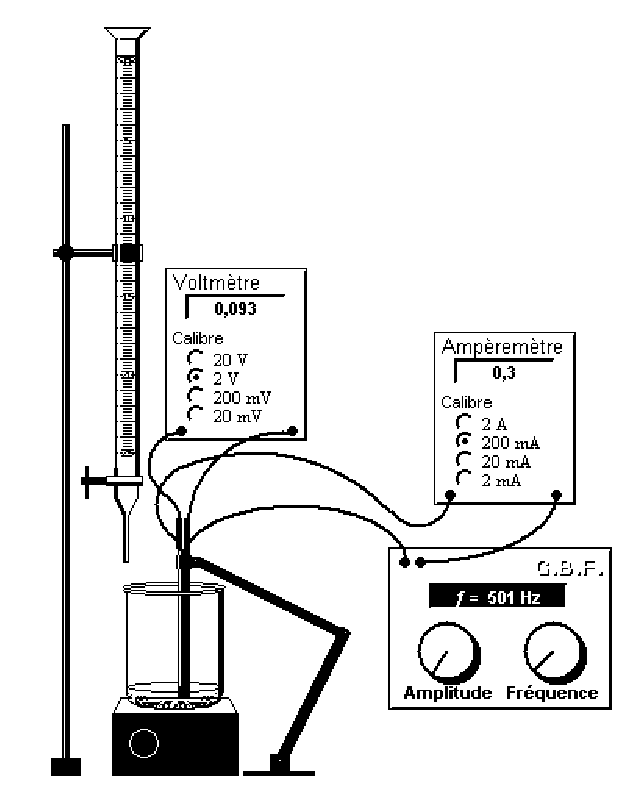
\includegraphics[width=6cm]{tp_prem_s_chimie/tp6_determination_par_conductimetrie_concentration/montage_conductimetrie.png.eps}
\caption{Dispositif exp�rimental}
\end{figure}
\end{center}


\end{multicols}



\subsection{R�sultats}
\begin{enumerate}
\item Calculer la conductance $G$ et compl�ter le tableau suivant.

\begin{arraydata}{6}
\hline
$V_0$ ($mL$)       &  0 &  5 & 10 & 15 & 20 & 25 \\ \hline
\rule[-0.4cm]{0cm}{1cm}
$C$ ($mol.L^{-1}$) &    &    &    &    &    &    \\ \hline
\rule[-0.4cm]{0cm}{1cm}
$G$ ($mS$)         &    &    &    &    &    &    \\ \hline
\end{arraydata}

\item Tracer la courbe d'�talonnage $G = f (C)$.
\end{enumerate}



\pagebreak
%\newpage


\section{D�termination de la concentration en $NaCl$ d'une solution de
  s�rum physiologique}

L'objectif est de d�terminer la concentration du chlorure de sodium dans le s�rum physiologique injectable.

\begin{enumerate}
\item Diluer au $1/100\ieme$ le s�rum physiologique. En pr�parer $500~mL$.

\item D�crire � l'aide de sch�mas le protocole utilis� pour r�aliser
  cette dilution au $1/100\ieme$ et obtenir la solution $S'$.

\item D�terminer la conductance $G'$ de cette solution $S'$.

\item En d�duire la concentration $C'$ du chlorure de sodium dans le
  s�rum physiologique dilu�.

\end{enumerate}


\vressort{3}

\section{Questions compl�mentaires}

%\begin{multicols}{2}

\begin{enumerate}
\item Expliquer comment calculer la concentration $C$ des diff�rentes
  solutions de chlorure de sodium. Donner l'expression de $C$ en
  fonction de $C_0$, $V_0$, $V$.


\item Comment calcule-t-on la conductance $G$ ?

\item Pour quelle raison pratique a-t-on int�r�t � prendre $U =
  1,00~V$ dans les diff�rentes manipulations ?

\item En extrapolant la courbe d'�talonnage, pr�voir la conductance
  d'une portion de solution concentr�e � $T = 58,4~g.L^{-1}$. Mesurer
  la conductance r�elle d'une portion d'une telle solution. Que
  peut-on conclure quant � la m�thode d'�talonnage utilis�e. On donne
  $M_{Na} = 23~g.mol^{-1}$ et $M_{Cl} = 35,5~g.mol^{-1}$.

\item Rappeler la valeur de la concentration $C'$ du chlorure de
  sodium dans le s�rum physiologique dilu�.

\item Comment peut-on alors d�terminer la concentration $C_0'$ du
  chlorure de sodium dans la solution commerciale de s�rum
  physiologique ? Calculer cette concentration $C_0'$ puis le titre
  massique (concentration massique) correspondant $T_0$. Le comparer avec
  les indications figurant sur l'�tiquette du flacon ($0,9~\%$ en masse).
\end{enumerate}


%\vressort{1}
\vressort{3}

\begin{center}
\begin{figure}[H]
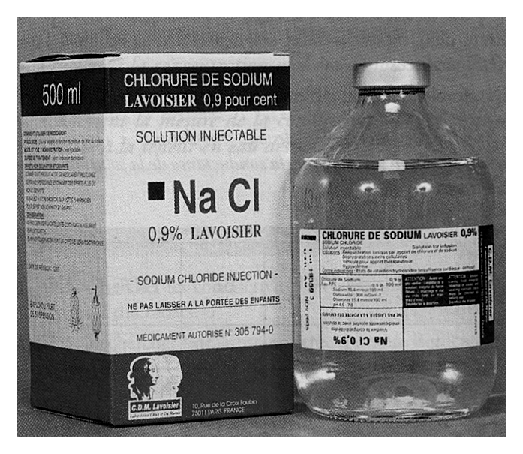
\includegraphics[width=7cm]{tp_prem_s_chimie/tp6_determination_par_conductimetrie_concentration/solution_nacl.png.eps}
\caption{Solution de chlorure de sodium}
\end{figure}
\end{center}


%\end{multicols}


\vressort{3} % cours elec circuit �lectrique

\tp{D�termination par conductim�trie\\
de la concentration en solut�\\
d'une solution ionique}


\begin{multicols}{2}

\objectifs{
\item r�aliser une courbe d'�talonnage $G = f(C)$ et en d�duire une
  concentration inconnue.
\item Aborder une limite de la m�thode d'�talonnage.
}
\vspace*{2cm}


\materiel{
\item b�cher $600~mL$
\item fiole jaug�e $500~mL$
\item burette gradu�e $25~mL$
\item pipette jaug�e $5~mL$
\item agitateur magn�tique.
\item solution de chlorure de sodium $S_0$ de concentration $C_0 =
  0,10~mol.L^{-1}$
\item flacon de s�rum physiologique
\item eau d�min�ralis�e
\item g�n�rateur basse fr�quence.
\item 2 multim�tres
\item cellule de conductim�trie.
}


\end{multicols}




\section{R�alisation d'une �chelle de conductance}


\begin{multicols}{2}

\subsection{Protocole op�ratoire}
\begin{enumerate}
\item Rincer la burette, la remplir � l'aide de la solution $S_0$ ajuster le
z�ro.

\item Avec la fiole jaug�e, introduire $V = 500~mL$ d'eau d�min�ralis�e dans
le b�cher.

\item Placer la cellule conductim�trique dans le b�cher et r�aliser le
montage �lectrique correspondant au sch�ma ci-contre. Les 2
multim�tres sont en mode alternatif ($AC$ ou \acsymbol).

\item Sur le GBF, r�gler la fr�quence $500~Hz$ et fixer la tension �
$1,00~V$.

\item Au contenu du b�cher, ajouter les volumes $V_0$ suivants de solution
de chlorure de sodium mesur�s pr�cis�ment gr�ce � la burette. Apr�s
chaque addition, v�rifier que la tension est toujours de $1,00~V$ et
relever la valeur de l'intensit�.

\end{enumerate}




\begin{center}
\begin{figure}[H]
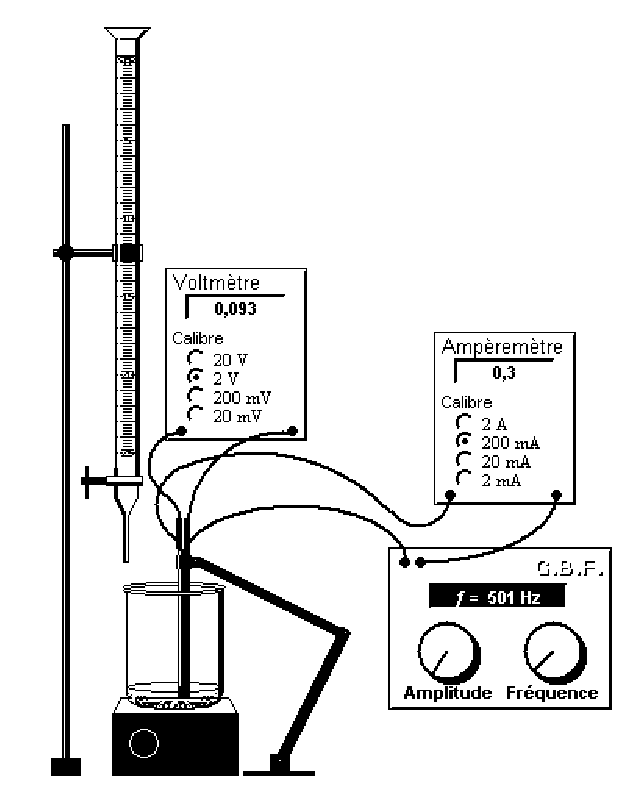
\includegraphics[width=6cm]{tp_prem_s_chimie/tp6_determination_par_conductimetrie_concentration/montage_conductimetrie.png.eps}
\caption{Dispositif exp�rimental}
\end{figure}
\end{center}


\end{multicols}



\subsection{R�sultats}
\begin{enumerate}
\item Calculer la conductance $G$ et compl�ter le tableau suivant.

\begin{arraydata}{6}
\hline
$V_0$ ($mL$)       &  0 &  5 & 10 & 15 & 20 & 25 \\ \hline
\rule[-0.4cm]{0cm}{1cm}
$C$ ($mol.L^{-1}$) &    &    &    &    &    &    \\ \hline
\rule[-0.4cm]{0cm}{1cm}
$G$ ($mS$)         &    &    &    &    &    &    \\ \hline
\end{arraydata}

\item Tracer la courbe d'�talonnage $G = f (C)$.
\end{enumerate}



\pagebreak
%\newpage


\section{D�termination de la concentration en $NaCl$ d'une solution de
  s�rum physiologique}

L'objectif est de d�terminer la concentration du chlorure de sodium dans le s�rum physiologique injectable.

\begin{enumerate}
\item Diluer au $1/100\ieme$ le s�rum physiologique. En pr�parer $500~mL$.

\item D�crire � l'aide de sch�mas le protocole utilis� pour r�aliser
  cette dilution au $1/100\ieme$ et obtenir la solution $S'$.

\item D�terminer la conductance $G'$ de cette solution $S'$.

\item En d�duire la concentration $C'$ du chlorure de sodium dans le
  s�rum physiologique dilu�.

\end{enumerate}


\vressort{3}

\section{Questions compl�mentaires}

%\begin{multicols}{2}

\begin{enumerate}
\item Expliquer comment calculer la concentration $C$ des diff�rentes
  solutions de chlorure de sodium. Donner l'expression de $C$ en
  fonction de $C_0$, $V_0$, $V$.


\item Comment calcule-t-on la conductance $G$ ?

\item Pour quelle raison pratique a-t-on int�r�t � prendre $U =
  1,00~V$ dans les diff�rentes manipulations ?

\item En extrapolant la courbe d'�talonnage, pr�voir la conductance
  d'une portion de solution concentr�e � $T = 58,4~g.L^{-1}$. Mesurer
  la conductance r�elle d'une portion d'une telle solution. Que
  peut-on conclure quant � la m�thode d'�talonnage utilis�e. On donne
  $M_{Na} = 23~g.mol^{-1}$ et $M_{Cl} = 35,5~g.mol^{-1}$.

\item Rappeler la valeur de la concentration $C'$ du chlorure de
  sodium dans le s�rum physiologique dilu�.

\item Comment peut-on alors d�terminer la concentration $C_0'$ du
  chlorure de sodium dans la solution commerciale de s�rum
  physiologique ? Calculer cette concentration $C_0'$ puis le titre
  massique (concentration massique) correspondant $T_0$. Le comparer avec
  les indications figurant sur l'�tiquette du flacon ($0,9~\%$ en masse).
\end{enumerate}


%\vressort{1}
\vressort{3}

\begin{center}
\begin{figure}[H]
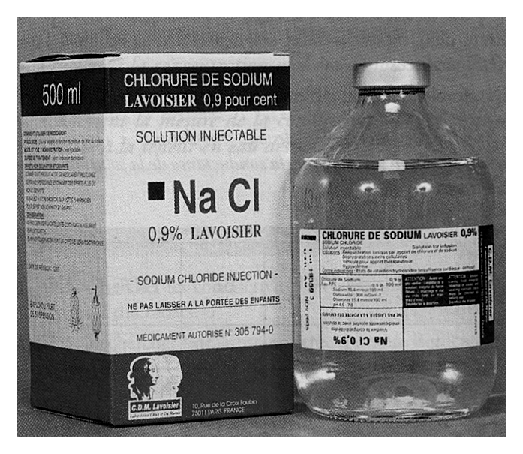
\includegraphics[width=7cm]{tp_prem_s_chimie/tp6_determination_par_conductimetrie_concentration/solution_nacl.png.eps}
\caption{Solution de chlorure de sodium}
\end{figure}
\end{center}


%\end{multicols}


\vressort{3} % tp mesure de tension et d'intensit�

\tp{D�termination par conductim�trie\\
de la concentration en solut�\\
d'une solution ionique}


\begin{multicols}{2}

\objectifs{
\item r�aliser une courbe d'�talonnage $G = f(C)$ et en d�duire une
  concentration inconnue.
\item Aborder une limite de la m�thode d'�talonnage.
}
\vspace*{2cm}


\materiel{
\item b�cher $600~mL$
\item fiole jaug�e $500~mL$
\item burette gradu�e $25~mL$
\item pipette jaug�e $5~mL$
\item agitateur magn�tique.
\item solution de chlorure de sodium $S_0$ de concentration $C_0 =
  0,10~mol.L^{-1}$
\item flacon de s�rum physiologique
\item eau d�min�ralis�e
\item g�n�rateur basse fr�quence.
\item 2 multim�tres
\item cellule de conductim�trie.
}


\end{multicols}




\section{R�alisation d'une �chelle de conductance}


\begin{multicols}{2}

\subsection{Protocole op�ratoire}
\begin{enumerate}
\item Rincer la burette, la remplir � l'aide de la solution $S_0$ ajuster le
z�ro.

\item Avec la fiole jaug�e, introduire $V = 500~mL$ d'eau d�min�ralis�e dans
le b�cher.

\item Placer la cellule conductim�trique dans le b�cher et r�aliser le
montage �lectrique correspondant au sch�ma ci-contre. Les 2
multim�tres sont en mode alternatif ($AC$ ou \acsymbol).

\item Sur le GBF, r�gler la fr�quence $500~Hz$ et fixer la tension �
$1,00~V$.

\item Au contenu du b�cher, ajouter les volumes $V_0$ suivants de solution
de chlorure de sodium mesur�s pr�cis�ment gr�ce � la burette. Apr�s
chaque addition, v�rifier que la tension est toujours de $1,00~V$ et
relever la valeur de l'intensit�.

\end{enumerate}




\begin{center}
\begin{figure}[H]
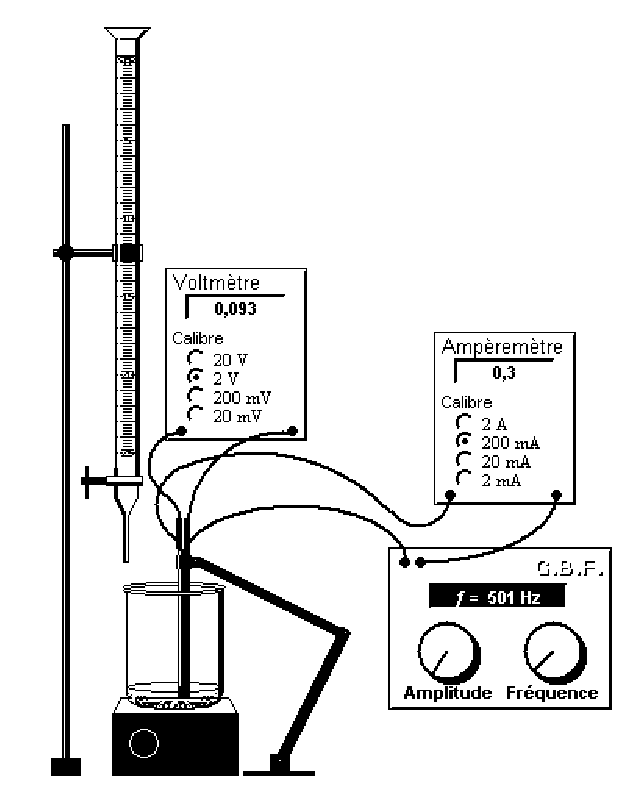
\includegraphics[width=6cm]{tp_prem_s_chimie/tp6_determination_par_conductimetrie_concentration/montage_conductimetrie.png.eps}
\caption{Dispositif exp�rimental}
\end{figure}
\end{center}


\end{multicols}



\subsection{R�sultats}
\begin{enumerate}
\item Calculer la conductance $G$ et compl�ter le tableau suivant.

\begin{arraydata}{6}
\hline
$V_0$ ($mL$)       &  0 &  5 & 10 & 15 & 20 & 25 \\ \hline
\rule[-0.4cm]{0cm}{1cm}
$C$ ($mol.L^{-1}$) &    &    &    &    &    &    \\ \hline
\rule[-0.4cm]{0cm}{1cm}
$G$ ($mS$)         &    &    &    &    &    &    \\ \hline
\end{arraydata}

\item Tracer la courbe d'�talonnage $G = f (C)$.
\end{enumerate}



\pagebreak
%\newpage


\section{D�termination de la concentration en $NaCl$ d'une solution de
  s�rum physiologique}

L'objectif est de d�terminer la concentration du chlorure de sodium dans le s�rum physiologique injectable.

\begin{enumerate}
\item Diluer au $1/100\ieme$ le s�rum physiologique. En pr�parer $500~mL$.

\item D�crire � l'aide de sch�mas le protocole utilis� pour r�aliser
  cette dilution au $1/100\ieme$ et obtenir la solution $S'$.

\item D�terminer la conductance $G'$ de cette solution $S'$.

\item En d�duire la concentration $C'$ du chlorure de sodium dans le
  s�rum physiologique dilu�.

\end{enumerate}


\vressort{3}

\section{Questions compl�mentaires}

%\begin{multicols}{2}

\begin{enumerate}
\item Expliquer comment calculer la concentration $C$ des diff�rentes
  solutions de chlorure de sodium. Donner l'expression de $C$ en
  fonction de $C_0$, $V_0$, $V$.


\item Comment calcule-t-on la conductance $G$ ?

\item Pour quelle raison pratique a-t-on int�r�t � prendre $U =
  1,00~V$ dans les diff�rentes manipulations ?

\item En extrapolant la courbe d'�talonnage, pr�voir la conductance
  d'une portion de solution concentr�e � $T = 58,4~g.L^{-1}$. Mesurer
  la conductance r�elle d'une portion d'une telle solution. Que
  peut-on conclure quant � la m�thode d'�talonnage utilis�e. On donne
  $M_{Na} = 23~g.mol^{-1}$ et $M_{Cl} = 35,5~g.mol^{-1}$.

\item Rappeler la valeur de la concentration $C'$ du chlorure de
  sodium dans le s�rum physiologique dilu�.

\item Comment peut-on alors d�terminer la concentration $C_0'$ du
  chlorure de sodium dans la solution commerciale de s�rum
  physiologique ? Calculer cette concentration $C_0'$ puis le titre
  massique (concentration massique) correspondant $T_0$. Le comparer avec
  les indications figurant sur l'�tiquette du flacon ($0,9~\%$ en masse).
\end{enumerate}


%\vressort{1}
\vressort{3}

\begin{center}
\begin{figure}[H]
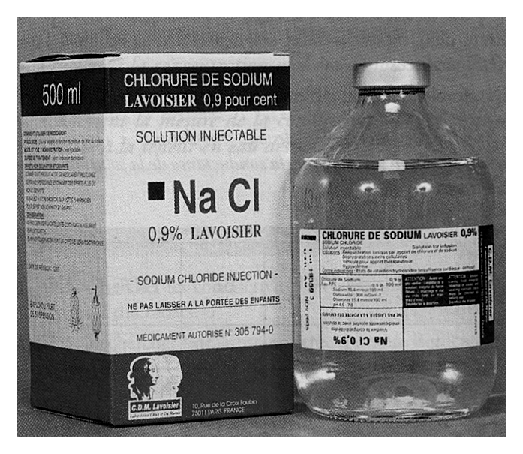
\includegraphics[width=7cm]{tp_prem_s_chimie/tp6_determination_par_conductimetrie_concentration/solution_nacl.png.eps}
\caption{Solution de chlorure de sodium}
\end{figure}
\end{center}


%\end{multicols}


\vressort{3} % document fiche
    % m�thode montage
    % utilisation d'un multim�tre, ...

\tp{D�termination par conductim�trie\\
de la concentration en solut�\\
d'une solution ionique}


\begin{multicols}{2}

\objectifs{
\item r�aliser une courbe d'�talonnage $G = f(C)$ et en d�duire une
  concentration inconnue.
\item Aborder une limite de la m�thode d'�talonnage.
}
\vspace*{2cm}


\materiel{
\item b�cher $600~mL$
\item fiole jaug�e $500~mL$
\item burette gradu�e $25~mL$
\item pipette jaug�e $5~mL$
\item agitateur magn�tique.
\item solution de chlorure de sodium $S_0$ de concentration $C_0 =
  0,10~mol.L^{-1}$
\item flacon de s�rum physiologique
\item eau d�min�ralis�e
\item g�n�rateur basse fr�quence.
\item 2 multim�tres
\item cellule de conductim�trie.
}


\end{multicols}




\section{R�alisation d'une �chelle de conductance}


\begin{multicols}{2}

\subsection{Protocole op�ratoire}
\begin{enumerate}
\item Rincer la burette, la remplir � l'aide de la solution $S_0$ ajuster le
z�ro.

\item Avec la fiole jaug�e, introduire $V = 500~mL$ d'eau d�min�ralis�e dans
le b�cher.

\item Placer la cellule conductim�trique dans le b�cher et r�aliser le
montage �lectrique correspondant au sch�ma ci-contre. Les 2
multim�tres sont en mode alternatif ($AC$ ou \acsymbol).

\item Sur le GBF, r�gler la fr�quence $500~Hz$ et fixer la tension �
$1,00~V$.

\item Au contenu du b�cher, ajouter les volumes $V_0$ suivants de solution
de chlorure de sodium mesur�s pr�cis�ment gr�ce � la burette. Apr�s
chaque addition, v�rifier que la tension est toujours de $1,00~V$ et
relever la valeur de l'intensit�.

\end{enumerate}




\begin{center}
\begin{figure}[H]
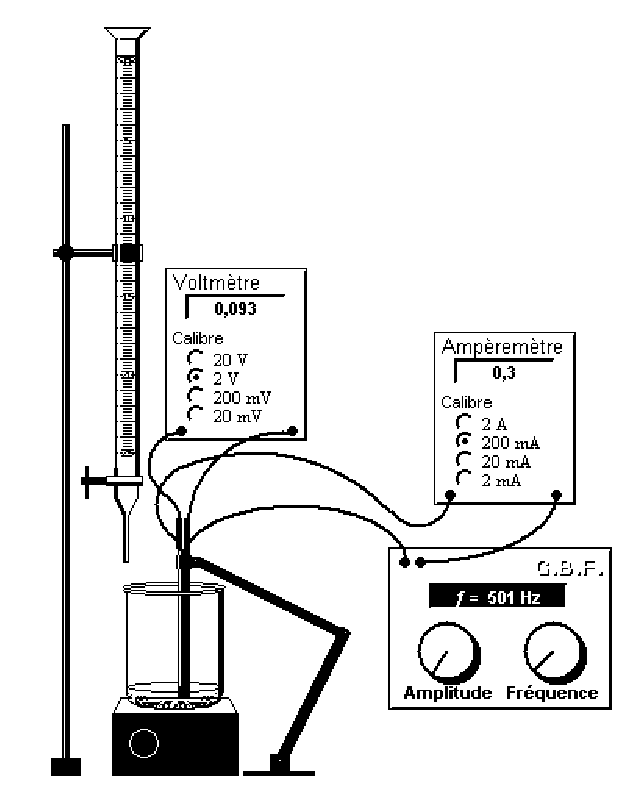
\includegraphics[width=6cm]{tp_prem_s_chimie/tp6_determination_par_conductimetrie_concentration/montage_conductimetrie.png.eps}
\caption{Dispositif exp�rimental}
\end{figure}
\end{center}


\end{multicols}



\subsection{R�sultats}
\begin{enumerate}
\item Calculer la conductance $G$ et compl�ter le tableau suivant.

\begin{arraydata}{6}
\hline
$V_0$ ($mL$)       &  0 &  5 & 10 & 15 & 20 & 25 \\ \hline
\rule[-0.4cm]{0cm}{1cm}
$C$ ($mol.L^{-1}$) &    &    &    &    &    &    \\ \hline
\rule[-0.4cm]{0cm}{1cm}
$G$ ($mS$)         &    &    &    &    &    &    \\ \hline
\end{arraydata}

\item Tracer la courbe d'�talonnage $G = f (C)$.
\end{enumerate}



\pagebreak
%\newpage


\section{D�termination de la concentration en $NaCl$ d'une solution de
  s�rum physiologique}

L'objectif est de d�terminer la concentration du chlorure de sodium dans le s�rum physiologique injectable.

\begin{enumerate}
\item Diluer au $1/100\ieme$ le s�rum physiologique. En pr�parer $500~mL$.

\item D�crire � l'aide de sch�mas le protocole utilis� pour r�aliser
  cette dilution au $1/100\ieme$ et obtenir la solution $S'$.

\item D�terminer la conductance $G'$ de cette solution $S'$.

\item En d�duire la concentration $C'$ du chlorure de sodium dans le
  s�rum physiologique dilu�.

\end{enumerate}


\vressort{3}

\section{Questions compl�mentaires}

%\begin{multicols}{2}

\begin{enumerate}
\item Expliquer comment calculer la concentration $C$ des diff�rentes
  solutions de chlorure de sodium. Donner l'expression de $C$ en
  fonction de $C_0$, $V_0$, $V$.


\item Comment calcule-t-on la conductance $G$ ?

\item Pour quelle raison pratique a-t-on int�r�t � prendre $U =
  1,00~V$ dans les diff�rentes manipulations ?

\item En extrapolant la courbe d'�talonnage, pr�voir la conductance
  d'une portion de solution concentr�e � $T = 58,4~g.L^{-1}$. Mesurer
  la conductance r�elle d'une portion d'une telle solution. Que
  peut-on conclure quant � la m�thode d'�talonnage utilis�e. On donne
  $M_{Na} = 23~g.mol^{-1}$ et $M_{Cl} = 35,5~g.mol^{-1}$.

\item Rappeler la valeur de la concentration $C'$ du chlorure de
  sodium dans le s�rum physiologique dilu�.

\item Comment peut-on alors d�terminer la concentration $C_0'$ du
  chlorure de sodium dans la solution commerciale de s�rum
  physiologique ? Calculer cette concentration $C_0'$ puis le titre
  massique (concentration massique) correspondant $T_0$. Le comparer avec
  les indications figurant sur l'�tiquette du flacon ($0,9~\%$ en masse).
\end{enumerate}


%\vressort{1}
\vressort{3}

\begin{center}
\begin{figure}[H]
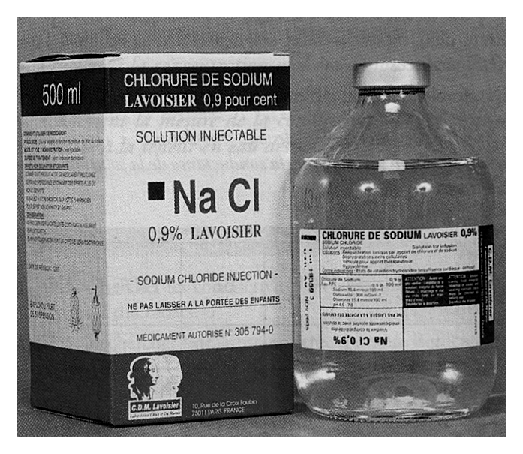
\includegraphics[width=7cm]{tp_prem_s_chimie/tp6_determination_par_conductimetrie_concentration/solution_nacl.png.eps}
\caption{Solution de chlorure de sodium}
\end{figure}
\end{center}


%\end{multicols}


\vressort{3} % tp loi d'ohm

\tp{D�termination par conductim�trie\\
de la concentration en solut�\\
d'une solution ionique}


\begin{multicols}{2}

\objectifs{
\item r�aliser une courbe d'�talonnage $G = f(C)$ et en d�duire une
  concentration inconnue.
\item Aborder une limite de la m�thode d'�talonnage.
}
\vspace*{2cm}


\materiel{
\item b�cher $600~mL$
\item fiole jaug�e $500~mL$
\item burette gradu�e $25~mL$
\item pipette jaug�e $5~mL$
\item agitateur magn�tique.
\item solution de chlorure de sodium $S_0$ de concentration $C_0 =
  0,10~mol.L^{-1}$
\item flacon de s�rum physiologique
\item eau d�min�ralis�e
\item g�n�rateur basse fr�quence.
\item 2 multim�tres
\item cellule de conductim�trie.
}


\end{multicols}




\section{R�alisation d'une �chelle de conductance}


\begin{multicols}{2}

\subsection{Protocole op�ratoire}
\begin{enumerate}
\item Rincer la burette, la remplir � l'aide de la solution $S_0$ ajuster le
z�ro.

\item Avec la fiole jaug�e, introduire $V = 500~mL$ d'eau d�min�ralis�e dans
le b�cher.

\item Placer la cellule conductim�trique dans le b�cher et r�aliser le
montage �lectrique correspondant au sch�ma ci-contre. Les 2
multim�tres sont en mode alternatif ($AC$ ou \acsymbol).

\item Sur le GBF, r�gler la fr�quence $500~Hz$ et fixer la tension �
$1,00~V$.

\item Au contenu du b�cher, ajouter les volumes $V_0$ suivants de solution
de chlorure de sodium mesur�s pr�cis�ment gr�ce � la burette. Apr�s
chaque addition, v�rifier que la tension est toujours de $1,00~V$ et
relever la valeur de l'intensit�.

\end{enumerate}




\begin{center}
\begin{figure}[H]
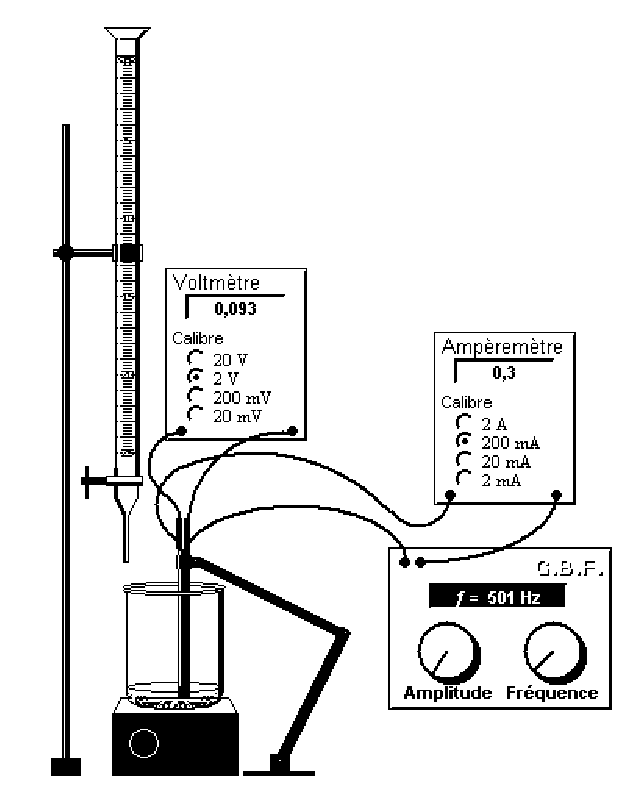
\includegraphics[width=6cm]{tp_prem_s_chimie/tp6_determination_par_conductimetrie_concentration/montage_conductimetrie.png.eps}
\caption{Dispositif exp�rimental}
\end{figure}
\end{center}


\end{multicols}



\subsection{R�sultats}
\begin{enumerate}
\item Calculer la conductance $G$ et compl�ter le tableau suivant.

\begin{arraydata}{6}
\hline
$V_0$ ($mL$)       &  0 &  5 & 10 & 15 & 20 & 25 \\ \hline
\rule[-0.4cm]{0cm}{1cm}
$C$ ($mol.L^{-1}$) &    &    &    &    &    &    \\ \hline
\rule[-0.4cm]{0cm}{1cm}
$G$ ($mS$)         &    &    &    &    &    &    \\ \hline
\end{arraydata}

\item Tracer la courbe d'�talonnage $G = f (C)$.
\end{enumerate}



\pagebreak
%\newpage


\section{D�termination de la concentration en $NaCl$ d'une solution de
  s�rum physiologique}

L'objectif est de d�terminer la concentration du chlorure de sodium dans le s�rum physiologique injectable.

\begin{enumerate}
\item Diluer au $1/100\ieme$ le s�rum physiologique. En pr�parer $500~mL$.

\item D�crire � l'aide de sch�mas le protocole utilis� pour r�aliser
  cette dilution au $1/100\ieme$ et obtenir la solution $S'$.

\item D�terminer la conductance $G'$ de cette solution $S'$.

\item En d�duire la concentration $C'$ du chlorure de sodium dans le
  s�rum physiologique dilu�.

\end{enumerate}


\vressort{3}

\section{Questions compl�mentaires}

%\begin{multicols}{2}

\begin{enumerate}
\item Expliquer comment calculer la concentration $C$ des diff�rentes
  solutions de chlorure de sodium. Donner l'expression de $C$ en
  fonction de $C_0$, $V_0$, $V$.


\item Comment calcule-t-on la conductance $G$ ?

\item Pour quelle raison pratique a-t-on int�r�t � prendre $U =
  1,00~V$ dans les diff�rentes manipulations ?

\item En extrapolant la courbe d'�talonnage, pr�voir la conductance
  d'une portion de solution concentr�e � $T = 58,4~g.L^{-1}$. Mesurer
  la conductance r�elle d'une portion d'une telle solution. Que
  peut-on conclure quant � la m�thode d'�talonnage utilis�e. On donne
  $M_{Na} = 23~g.mol^{-1}$ et $M_{Cl} = 35,5~g.mol^{-1}$.

\item Rappeler la valeur de la concentration $C'$ du chlorure de
  sodium dans le s�rum physiologique dilu�.

\item Comment peut-on alors d�terminer la concentration $C_0'$ du
  chlorure de sodium dans la solution commerciale de s�rum
  physiologique ? Calculer cette concentration $C_0'$ puis le titre
  massique (concentration massique) correspondant $T_0$. Le comparer avec
  les indications figurant sur l'�tiquette du flacon ($0,9~\%$ en masse).
\end{enumerate}


%\vressort{1}
\vressort{3}

\begin{center}
\begin{figure}[H]
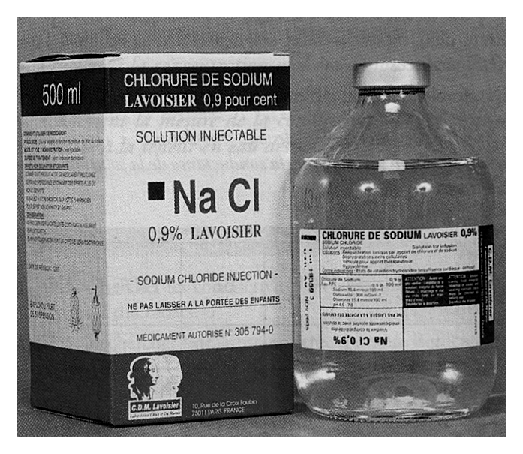
\includegraphics[width=7cm]{tp_prem_s_chimie/tp6_determination_par_conductimetrie_concentration/solution_nacl.png.eps}
\caption{Solution de chlorure de sodium}
\end{figure}
\end{center}


%\end{multicols}


\vressort{3} % tp associations de R

% association r s�rie (trac� U en fonction de I et montrer qu'on ajoute U)
% association r parall�le (trac� U en fonction de I et montrer qu'on ajoute I)

%\chapitre{G�n�rateurs et r�cepteurs}
%\tp{D�termination par conductim�trie\\
de la concentration en solut�\\
d'une solution ionique}


\begin{multicols}{2}

\objectifs{
\item r�aliser une courbe d'�talonnage $G = f(C)$ et en d�duire une
  concentration inconnue.
\item Aborder une limite de la m�thode d'�talonnage.
}
\vspace*{2cm}


\materiel{
\item b�cher $600~mL$
\item fiole jaug�e $500~mL$
\item burette gradu�e $25~mL$
\item pipette jaug�e $5~mL$
\item agitateur magn�tique.
\item solution de chlorure de sodium $S_0$ de concentration $C_0 =
  0,10~mol.L^{-1}$
\item flacon de s�rum physiologique
\item eau d�min�ralis�e
\item g�n�rateur basse fr�quence.
\item 2 multim�tres
\item cellule de conductim�trie.
}


\end{multicols}




\section{R�alisation d'une �chelle de conductance}


\begin{multicols}{2}

\subsection{Protocole op�ratoire}
\begin{enumerate}
\item Rincer la burette, la remplir � l'aide de la solution $S_0$ ajuster le
z�ro.

\item Avec la fiole jaug�e, introduire $V = 500~mL$ d'eau d�min�ralis�e dans
le b�cher.

\item Placer la cellule conductim�trique dans le b�cher et r�aliser le
montage �lectrique correspondant au sch�ma ci-contre. Les 2
multim�tres sont en mode alternatif ($AC$ ou \acsymbol).

\item Sur le GBF, r�gler la fr�quence $500~Hz$ et fixer la tension �
$1,00~V$.

\item Au contenu du b�cher, ajouter les volumes $V_0$ suivants de solution
de chlorure de sodium mesur�s pr�cis�ment gr�ce � la burette. Apr�s
chaque addition, v�rifier que la tension est toujours de $1,00~V$ et
relever la valeur de l'intensit�.

\end{enumerate}




\begin{center}
\begin{figure}[H]
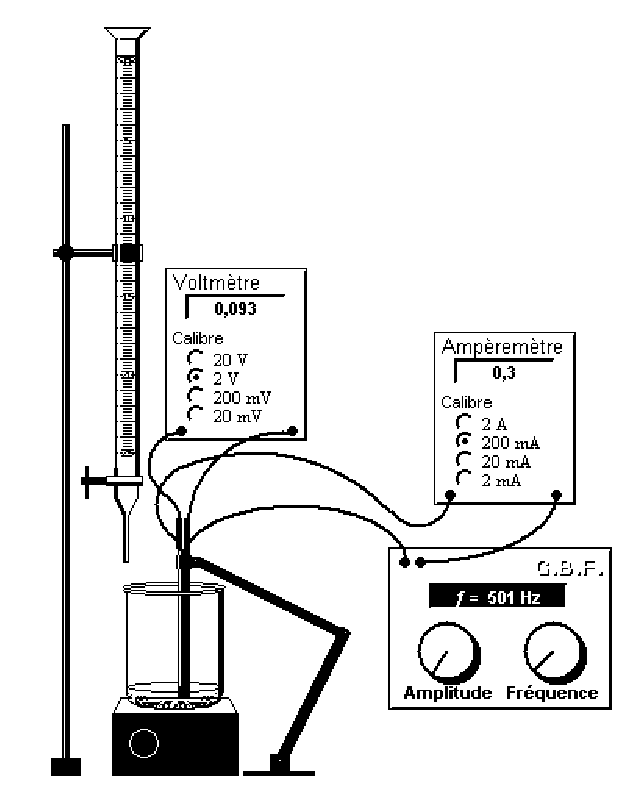
\includegraphics[width=6cm]{tp_prem_s_chimie/tp6_determination_par_conductimetrie_concentration/montage_conductimetrie.png.eps}
\caption{Dispositif exp�rimental}
\end{figure}
\end{center}


\end{multicols}



\subsection{R�sultats}
\begin{enumerate}
\item Calculer la conductance $G$ et compl�ter le tableau suivant.

\begin{arraydata}{6}
\hline
$V_0$ ($mL$)       &  0 &  5 & 10 & 15 & 20 & 25 \\ \hline
\rule[-0.4cm]{0cm}{1cm}
$C$ ($mol.L^{-1}$) &    &    &    &    &    &    \\ \hline
\rule[-0.4cm]{0cm}{1cm}
$G$ ($mS$)         &    &    &    &    &    &    \\ \hline
\end{arraydata}

\item Tracer la courbe d'�talonnage $G = f (C)$.
\end{enumerate}



\pagebreak
%\newpage


\section{D�termination de la concentration en $NaCl$ d'une solution de
  s�rum physiologique}

L'objectif est de d�terminer la concentration du chlorure de sodium dans le s�rum physiologique injectable.

\begin{enumerate}
\item Diluer au $1/100\ieme$ le s�rum physiologique. En pr�parer $500~mL$.

\item D�crire � l'aide de sch�mas le protocole utilis� pour r�aliser
  cette dilution au $1/100\ieme$ et obtenir la solution $S'$.

\item D�terminer la conductance $G'$ de cette solution $S'$.

\item En d�duire la concentration $C'$ du chlorure de sodium dans le
  s�rum physiologique dilu�.

\end{enumerate}


\vressort{3}

\section{Questions compl�mentaires}

%\begin{multicols}{2}

\begin{enumerate}
\item Expliquer comment calculer la concentration $C$ des diff�rentes
  solutions de chlorure de sodium. Donner l'expression de $C$ en
  fonction de $C_0$, $V_0$, $V$.


\item Comment calcule-t-on la conductance $G$ ?

\item Pour quelle raison pratique a-t-on int�r�t � prendre $U =
  1,00~V$ dans les diff�rentes manipulations ?

\item En extrapolant la courbe d'�talonnage, pr�voir la conductance
  d'une portion de solution concentr�e � $T = 58,4~g.L^{-1}$. Mesurer
  la conductance r�elle d'une portion d'une telle solution. Que
  peut-on conclure quant � la m�thode d'�talonnage utilis�e. On donne
  $M_{Na} = 23~g.mol^{-1}$ et $M_{Cl} = 35,5~g.mol^{-1}$.

\item Rappeler la valeur de la concentration $C'$ du chlorure de
  sodium dans le s�rum physiologique dilu�.

\item Comment peut-on alors d�terminer la concentration $C_0'$ du
  chlorure de sodium dans la solution commerciale de s�rum
  physiologique ? Calculer cette concentration $C_0'$ puis le titre
  massique (concentration massique) correspondant $T_0$. Le comparer avec
  les indications figurant sur l'�tiquette du flacon ($0,9~\%$ en masse).
\end{enumerate}


%\vressort{1}
\vressort{3}

\begin{center}
\begin{figure}[H]
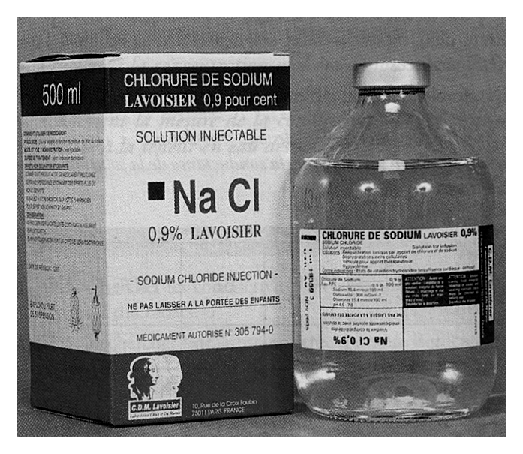
\includegraphics[width=7cm]{tp_prem_s_chimie/tp6_determination_par_conductimetrie_concentration/solution_nacl.png.eps}
\caption{Solution de chlorure de sodium}
\end{figure}
\end{center}


%\end{multicols}


\vressort{3} % cours elec g�n�rateurs, r�cepteurs

%\tp{D�termination par conductim�trie\\
de la concentration en solut�\\
d'une solution ionique}


\begin{multicols}{2}

\objectifs{
\item r�aliser une courbe d'�talonnage $G = f(C)$ et en d�duire une
  concentration inconnue.
\item Aborder une limite de la m�thode d'�talonnage.
}
\vspace*{2cm}


\materiel{
\item b�cher $600~mL$
\item fiole jaug�e $500~mL$
\item burette gradu�e $25~mL$
\item pipette jaug�e $5~mL$
\item agitateur magn�tique.
\item solution de chlorure de sodium $S_0$ de concentration $C_0 =
  0,10~mol.L^{-1}$
\item flacon de s�rum physiologique
\item eau d�min�ralis�e
\item g�n�rateur basse fr�quence.
\item 2 multim�tres
\item cellule de conductim�trie.
}


\end{multicols}




\section{R�alisation d'une �chelle de conductance}


\begin{multicols}{2}

\subsection{Protocole op�ratoire}
\begin{enumerate}
\item Rincer la burette, la remplir � l'aide de la solution $S_0$ ajuster le
z�ro.

\item Avec la fiole jaug�e, introduire $V = 500~mL$ d'eau d�min�ralis�e dans
le b�cher.

\item Placer la cellule conductim�trique dans le b�cher et r�aliser le
montage �lectrique correspondant au sch�ma ci-contre. Les 2
multim�tres sont en mode alternatif ($AC$ ou \acsymbol).

\item Sur le GBF, r�gler la fr�quence $500~Hz$ et fixer la tension �
$1,00~V$.

\item Au contenu du b�cher, ajouter les volumes $V_0$ suivants de solution
de chlorure de sodium mesur�s pr�cis�ment gr�ce � la burette. Apr�s
chaque addition, v�rifier que la tension est toujours de $1,00~V$ et
relever la valeur de l'intensit�.

\end{enumerate}




\begin{center}
\begin{figure}[H]
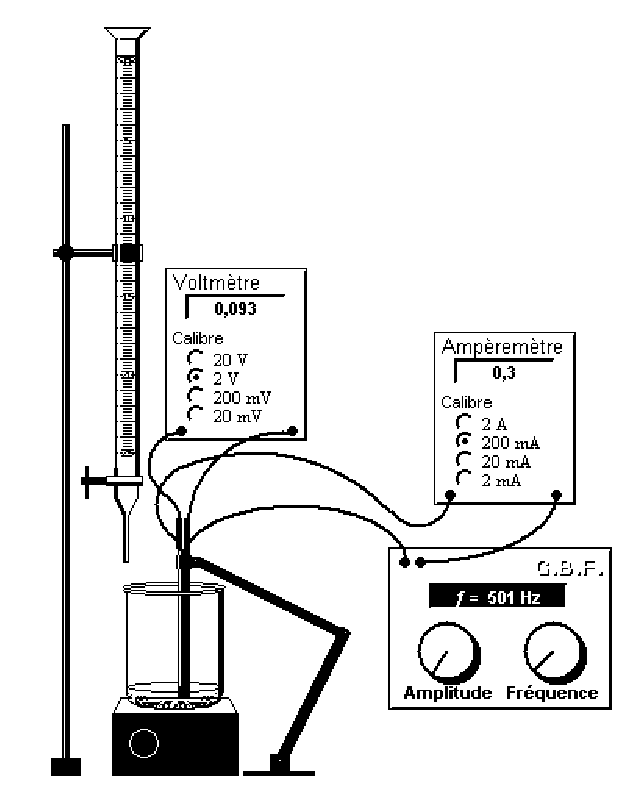
\includegraphics[width=6cm]{tp_prem_s_chimie/tp6_determination_par_conductimetrie_concentration/montage_conductimetrie.png.eps}
\caption{Dispositif exp�rimental}
\end{figure}
\end{center}


\end{multicols}



\subsection{R�sultats}
\begin{enumerate}
\item Calculer la conductance $G$ et compl�ter le tableau suivant.

\begin{arraydata}{6}
\hline
$V_0$ ($mL$)       &  0 &  5 & 10 & 15 & 20 & 25 \\ \hline
\rule[-0.4cm]{0cm}{1cm}
$C$ ($mol.L^{-1}$) &    &    &    &    &    &    \\ \hline
\rule[-0.4cm]{0cm}{1cm}
$G$ ($mS$)         &    &    &    &    &    &    \\ \hline
\end{arraydata}

\item Tracer la courbe d'�talonnage $G = f (C)$.
\end{enumerate}



\pagebreak
%\newpage


\section{D�termination de la concentration en $NaCl$ d'une solution de
  s�rum physiologique}

L'objectif est de d�terminer la concentration du chlorure de sodium dans le s�rum physiologique injectable.

\begin{enumerate}
\item Diluer au $1/100\ieme$ le s�rum physiologique. En pr�parer $500~mL$.

\item D�crire � l'aide de sch�mas le protocole utilis� pour r�aliser
  cette dilution au $1/100\ieme$ et obtenir la solution $S'$.

\item D�terminer la conductance $G'$ de cette solution $S'$.

\item En d�duire la concentration $C'$ du chlorure de sodium dans le
  s�rum physiologique dilu�.

\end{enumerate}


\vressort{3}

\section{Questions compl�mentaires}

%\begin{multicols}{2}

\begin{enumerate}
\item Expliquer comment calculer la concentration $C$ des diff�rentes
  solutions de chlorure de sodium. Donner l'expression de $C$ en
  fonction de $C_0$, $V_0$, $V$.


\item Comment calcule-t-on la conductance $G$ ?

\item Pour quelle raison pratique a-t-on int�r�t � prendre $U =
  1,00~V$ dans les diff�rentes manipulations ?

\item En extrapolant la courbe d'�talonnage, pr�voir la conductance
  d'une portion de solution concentr�e � $T = 58,4~g.L^{-1}$. Mesurer
  la conductance r�elle d'une portion d'une telle solution. Que
  peut-on conclure quant � la m�thode d'�talonnage utilis�e. On donne
  $M_{Na} = 23~g.mol^{-1}$ et $M_{Cl} = 35,5~g.mol^{-1}$.

\item Rappeler la valeur de la concentration $C'$ du chlorure de
  sodium dans le s�rum physiologique dilu�.

\item Comment peut-on alors d�terminer la concentration $C_0'$ du
  chlorure de sodium dans la solution commerciale de s�rum
  physiologique ? Calculer cette concentration $C_0'$ puis le titre
  massique (concentration massique) correspondant $T_0$. Le comparer avec
  les indications figurant sur l'�tiquette du flacon ($0,9~\%$ en masse).
\end{enumerate}


%\vressort{1}
\vressort{3}

\begin{center}
\begin{figure}[H]
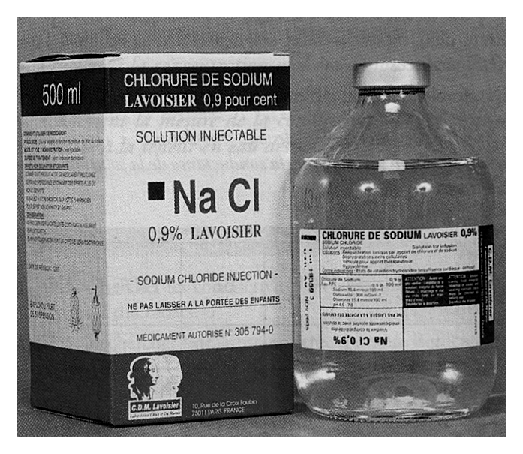
\includegraphics[width=7cm]{tp_prem_s_chimie/tp6_determination_par_conductimetrie_concentration/solution_nacl.png.eps}
\caption{Solution de chlorure de sodium}
\end{figure}
\end{center}


%\end{multicols}


\vressort{3} % tp caract�ristique d'un g�n�rateur
%\tp{D�termination par conductim�trie\\
de la concentration en solut�\\
d'une solution ionique}


\begin{multicols}{2}

\objectifs{
\item r�aliser une courbe d'�talonnage $G = f(C)$ et en d�duire une
  concentration inconnue.
\item Aborder une limite de la m�thode d'�talonnage.
}
\vspace*{2cm}


\materiel{
\item b�cher $600~mL$
\item fiole jaug�e $500~mL$
\item burette gradu�e $25~mL$
\item pipette jaug�e $5~mL$
\item agitateur magn�tique.
\item solution de chlorure de sodium $S_0$ de concentration $C_0 =
  0,10~mol.L^{-1}$
\item flacon de s�rum physiologique
\item eau d�min�ralis�e
\item g�n�rateur basse fr�quence.
\item 2 multim�tres
\item cellule de conductim�trie.
}


\end{multicols}




\section{R�alisation d'une �chelle de conductance}


\begin{multicols}{2}

\subsection{Protocole op�ratoire}
\begin{enumerate}
\item Rincer la burette, la remplir � l'aide de la solution $S_0$ ajuster le
z�ro.

\item Avec la fiole jaug�e, introduire $V = 500~mL$ d'eau d�min�ralis�e dans
le b�cher.

\item Placer la cellule conductim�trique dans le b�cher et r�aliser le
montage �lectrique correspondant au sch�ma ci-contre. Les 2
multim�tres sont en mode alternatif ($AC$ ou \acsymbol).

\item Sur le GBF, r�gler la fr�quence $500~Hz$ et fixer la tension �
$1,00~V$.

\item Au contenu du b�cher, ajouter les volumes $V_0$ suivants de solution
de chlorure de sodium mesur�s pr�cis�ment gr�ce � la burette. Apr�s
chaque addition, v�rifier que la tension est toujours de $1,00~V$ et
relever la valeur de l'intensit�.

\end{enumerate}




\begin{center}
\begin{figure}[H]
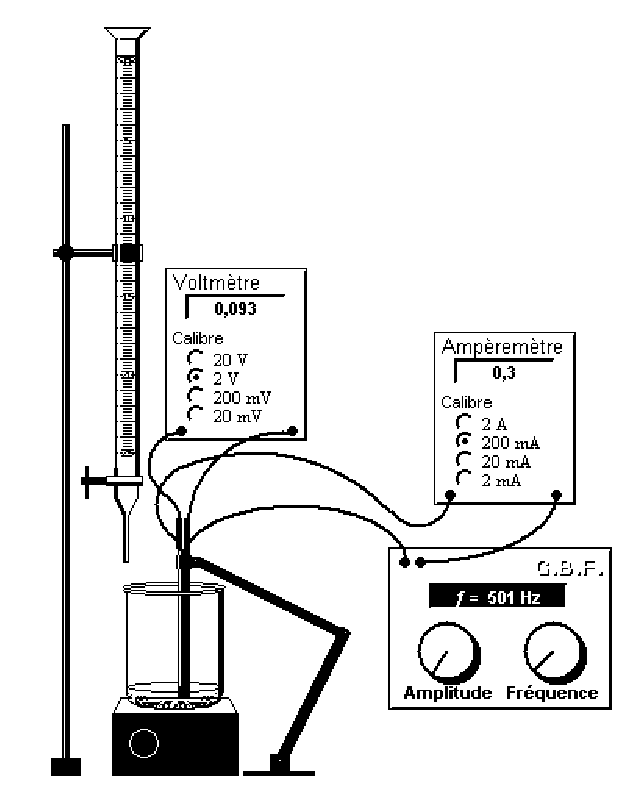
\includegraphics[width=6cm]{tp_prem_s_chimie/tp6_determination_par_conductimetrie_concentration/montage_conductimetrie.png.eps}
\caption{Dispositif exp�rimental}
\end{figure}
\end{center}


\end{multicols}



\subsection{R�sultats}
\begin{enumerate}
\item Calculer la conductance $G$ et compl�ter le tableau suivant.

\begin{arraydata}{6}
\hline
$V_0$ ($mL$)       &  0 &  5 & 10 & 15 & 20 & 25 \\ \hline
\rule[-0.4cm]{0cm}{1cm}
$C$ ($mol.L^{-1}$) &    &    &    &    &    &    \\ \hline
\rule[-0.4cm]{0cm}{1cm}
$G$ ($mS$)         &    &    &    &    &    &    \\ \hline
\end{arraydata}

\item Tracer la courbe d'�talonnage $G = f (C)$.
\end{enumerate}



\pagebreak
%\newpage


\section{D�termination de la concentration en $NaCl$ d'une solution de
  s�rum physiologique}

L'objectif est de d�terminer la concentration du chlorure de sodium dans le s�rum physiologique injectable.

\begin{enumerate}
\item Diluer au $1/100\ieme$ le s�rum physiologique. En pr�parer $500~mL$.

\item D�crire � l'aide de sch�mas le protocole utilis� pour r�aliser
  cette dilution au $1/100\ieme$ et obtenir la solution $S'$.

\item D�terminer la conductance $G'$ de cette solution $S'$.

\item En d�duire la concentration $C'$ du chlorure de sodium dans le
  s�rum physiologique dilu�.

\end{enumerate}


\vressort{3}

\section{Questions compl�mentaires}

%\begin{multicols}{2}

\begin{enumerate}
\item Expliquer comment calculer la concentration $C$ des diff�rentes
  solutions de chlorure de sodium. Donner l'expression de $C$ en
  fonction de $C_0$, $V_0$, $V$.


\item Comment calcule-t-on la conductance $G$ ?

\item Pour quelle raison pratique a-t-on int�r�t � prendre $U =
  1,00~V$ dans les diff�rentes manipulations ?

\item En extrapolant la courbe d'�talonnage, pr�voir la conductance
  d'une portion de solution concentr�e � $T = 58,4~g.L^{-1}$. Mesurer
  la conductance r�elle d'une portion d'une telle solution. Que
  peut-on conclure quant � la m�thode d'�talonnage utilis�e. On donne
  $M_{Na} = 23~g.mol^{-1}$ et $M_{Cl} = 35,5~g.mol^{-1}$.

\item Rappeler la valeur de la concentration $C'$ du chlorure de
  sodium dans le s�rum physiologique dilu�.

\item Comment peut-on alors d�terminer la concentration $C_0'$ du
  chlorure de sodium dans la solution commerciale de s�rum
  physiologique ? Calculer cette concentration $C_0'$ puis le titre
  massique (concentration massique) correspondant $T_0$. Le comparer avec
  les indications figurant sur l'�tiquette du flacon ($0,9~\%$ en masse).
\end{enumerate}


%\vressort{1}
\vressort{3}

\begin{center}
\begin{figure}[H]
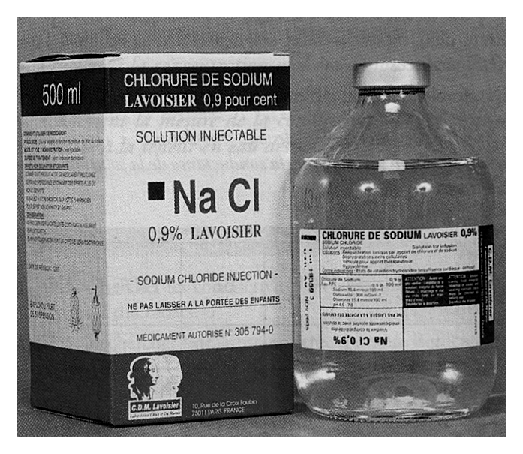
\includegraphics[width=7cm]{tp_prem_s_chimie/tp6_determination_par_conductimetrie_concentration/solution_nacl.png.eps}
\caption{Solution de chlorure de sodium}
\end{figure}
\end{center}


%\end{multicols}


\vressort{3} % tp caract�ristique d'un
                                % r�cepteur (�lectrolyseur)


\tp{D�termination par conductim�trie\\
de la concentration en solut�\\
d'une solution ionique}


\begin{multicols}{2}

\objectifs{
\item r�aliser une courbe d'�talonnage $G = f(C)$ et en d�duire une
  concentration inconnue.
\item Aborder une limite de la m�thode d'�talonnage.
}
\vspace*{2cm}


\materiel{
\item b�cher $600~mL$
\item fiole jaug�e $500~mL$
\item burette gradu�e $25~mL$
\item pipette jaug�e $5~mL$
\item agitateur magn�tique.
\item solution de chlorure de sodium $S_0$ de concentration $C_0 =
  0,10~mol.L^{-1}$
\item flacon de s�rum physiologique
\item eau d�min�ralis�e
\item g�n�rateur basse fr�quence.
\item 2 multim�tres
\item cellule de conductim�trie.
}


\end{multicols}




\section{R�alisation d'une �chelle de conductance}


\begin{multicols}{2}

\subsection{Protocole op�ratoire}
\begin{enumerate}
\item Rincer la burette, la remplir � l'aide de la solution $S_0$ ajuster le
z�ro.

\item Avec la fiole jaug�e, introduire $V = 500~mL$ d'eau d�min�ralis�e dans
le b�cher.

\item Placer la cellule conductim�trique dans le b�cher et r�aliser le
montage �lectrique correspondant au sch�ma ci-contre. Les 2
multim�tres sont en mode alternatif ($AC$ ou \acsymbol).

\item Sur le GBF, r�gler la fr�quence $500~Hz$ et fixer la tension �
$1,00~V$.

\item Au contenu du b�cher, ajouter les volumes $V_0$ suivants de solution
de chlorure de sodium mesur�s pr�cis�ment gr�ce � la burette. Apr�s
chaque addition, v�rifier que la tension est toujours de $1,00~V$ et
relever la valeur de l'intensit�.

\end{enumerate}




\begin{center}
\begin{figure}[H]
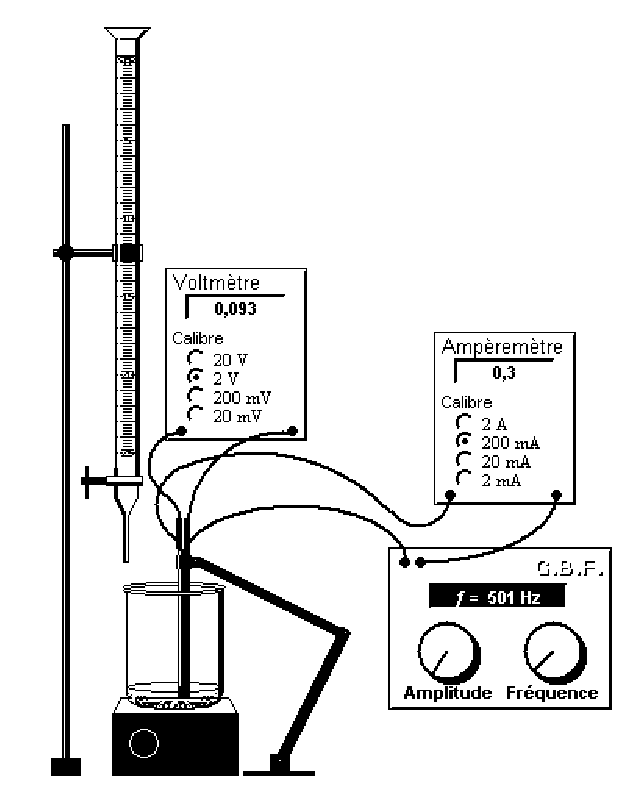
\includegraphics[width=6cm]{tp_prem_s_chimie/tp6_determination_par_conductimetrie_concentration/montage_conductimetrie.png.eps}
\caption{Dispositif exp�rimental}
\end{figure}
\end{center}


\end{multicols}



\subsection{R�sultats}
\begin{enumerate}
\item Calculer la conductance $G$ et compl�ter le tableau suivant.

\begin{arraydata}{6}
\hline
$V_0$ ($mL$)       &  0 &  5 & 10 & 15 & 20 & 25 \\ \hline
\rule[-0.4cm]{0cm}{1cm}
$C$ ($mol.L^{-1}$) &    &    &    &    &    &    \\ \hline
\rule[-0.4cm]{0cm}{1cm}
$G$ ($mS$)         &    &    &    &    &    &    \\ \hline
\end{arraydata}

\item Tracer la courbe d'�talonnage $G = f (C)$.
\end{enumerate}



\pagebreak
%\newpage


\section{D�termination de la concentration en $NaCl$ d'une solution de
  s�rum physiologique}

L'objectif est de d�terminer la concentration du chlorure de sodium dans le s�rum physiologique injectable.

\begin{enumerate}
\item Diluer au $1/100\ieme$ le s�rum physiologique. En pr�parer $500~mL$.

\item D�crire � l'aide de sch�mas le protocole utilis� pour r�aliser
  cette dilution au $1/100\ieme$ et obtenir la solution $S'$.

\item D�terminer la conductance $G'$ de cette solution $S'$.

\item En d�duire la concentration $C'$ du chlorure de sodium dans le
  s�rum physiologique dilu�.

\end{enumerate}


\vressort{3}

\section{Questions compl�mentaires}

%\begin{multicols}{2}

\begin{enumerate}
\item Expliquer comment calculer la concentration $C$ des diff�rentes
  solutions de chlorure de sodium. Donner l'expression de $C$ en
  fonction de $C_0$, $V_0$, $V$.


\item Comment calcule-t-on la conductance $G$ ?

\item Pour quelle raison pratique a-t-on int�r�t � prendre $U =
  1,00~V$ dans les diff�rentes manipulations ?

\item En extrapolant la courbe d'�talonnage, pr�voir la conductance
  d'une portion de solution concentr�e � $T = 58,4~g.L^{-1}$. Mesurer
  la conductance r�elle d'une portion d'une telle solution. Que
  peut-on conclure quant � la m�thode d'�talonnage utilis�e. On donne
  $M_{Na} = 23~g.mol^{-1}$ et $M_{Cl} = 35,5~g.mol^{-1}$.

\item Rappeler la valeur de la concentration $C'$ du chlorure de
  sodium dans le s�rum physiologique dilu�.

\item Comment peut-on alors d�terminer la concentration $C_0'$ du
  chlorure de sodium dans la solution commerciale de s�rum
  physiologique ? Calculer cette concentration $C_0'$ puis le titre
  massique (concentration massique) correspondant $T_0$. Le comparer avec
  les indications figurant sur l'�tiquette du flacon ($0,9~\%$ en masse).
\end{enumerate}


%\vressort{1}
\vressort{3}

\begin{center}
\begin{figure}[H]
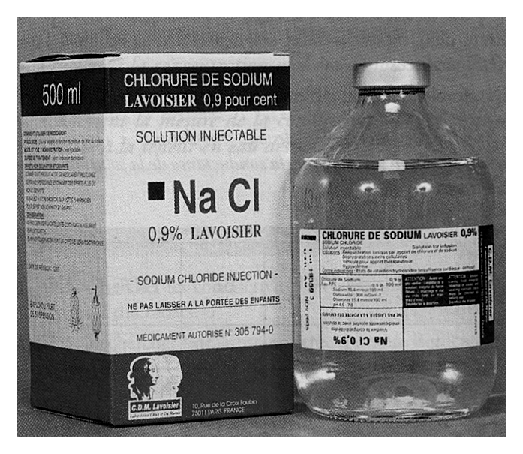
\includegraphics[width=7cm]{tp_prem_s_chimie/tp6_determination_par_conductimetrie_concentration/solution_nacl.png.eps}
\caption{Solution de chlorure de sodium}
\end{figure}
\end{center}


%\end{multicols}


\vressort{3} % tp puissance �nergie (continu)



\chapitre{Optique g�om�trique}
\tp{D�termination par conductim�trie\\
de la concentration en solut�\\
d'une solution ionique}


\begin{multicols}{2}

\objectifs{
\item r�aliser une courbe d'�talonnage $G = f(C)$ et en d�duire une
  concentration inconnue.
\item Aborder une limite de la m�thode d'�talonnage.
}
\vspace*{2cm}


\materiel{
\item b�cher $600~mL$
\item fiole jaug�e $500~mL$
\item burette gradu�e $25~mL$
\item pipette jaug�e $5~mL$
\item agitateur magn�tique.
\item solution de chlorure de sodium $S_0$ de concentration $C_0 =
  0,10~mol.L^{-1}$
\item flacon de s�rum physiologique
\item eau d�min�ralis�e
\item g�n�rateur basse fr�quence.
\item 2 multim�tres
\item cellule de conductim�trie.
}


\end{multicols}




\section{R�alisation d'une �chelle de conductance}


\begin{multicols}{2}

\subsection{Protocole op�ratoire}
\begin{enumerate}
\item Rincer la burette, la remplir � l'aide de la solution $S_0$ ajuster le
z�ro.

\item Avec la fiole jaug�e, introduire $V = 500~mL$ d'eau d�min�ralis�e dans
le b�cher.

\item Placer la cellule conductim�trique dans le b�cher et r�aliser le
montage �lectrique correspondant au sch�ma ci-contre. Les 2
multim�tres sont en mode alternatif ($AC$ ou \acsymbol).

\item Sur le GBF, r�gler la fr�quence $500~Hz$ et fixer la tension �
$1,00~V$.

\item Au contenu du b�cher, ajouter les volumes $V_0$ suivants de solution
de chlorure de sodium mesur�s pr�cis�ment gr�ce � la burette. Apr�s
chaque addition, v�rifier que la tension est toujours de $1,00~V$ et
relever la valeur de l'intensit�.

\end{enumerate}




\begin{center}
\begin{figure}[H]
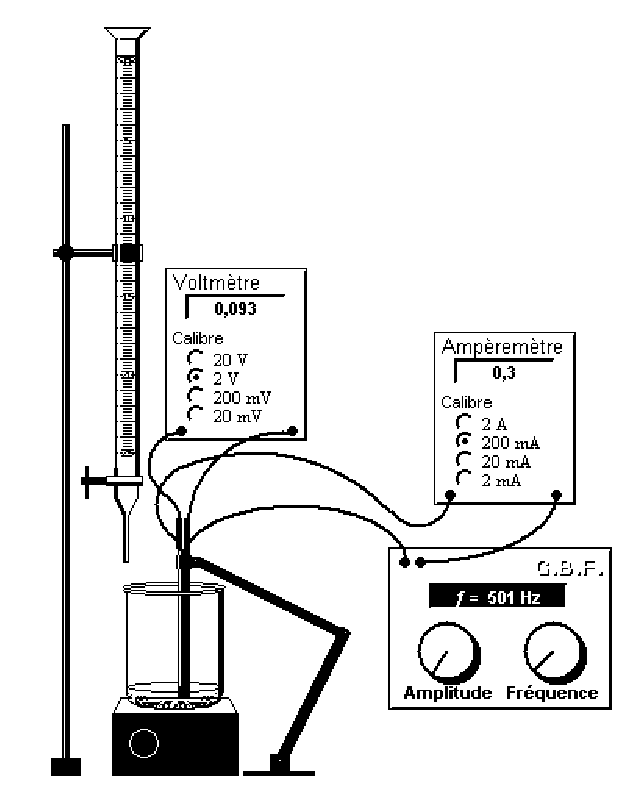
\includegraphics[width=6cm]{tp_prem_s_chimie/tp6_determination_par_conductimetrie_concentration/montage_conductimetrie.png.eps}
\caption{Dispositif exp�rimental}
\end{figure}
\end{center}


\end{multicols}



\subsection{R�sultats}
\begin{enumerate}
\item Calculer la conductance $G$ et compl�ter le tableau suivant.

\begin{arraydata}{6}
\hline
$V_0$ ($mL$)       &  0 &  5 & 10 & 15 & 20 & 25 \\ \hline
\rule[-0.4cm]{0cm}{1cm}
$C$ ($mol.L^{-1}$) &    &    &    &    &    &    \\ \hline
\rule[-0.4cm]{0cm}{1cm}
$G$ ($mS$)         &    &    &    &    &    &    \\ \hline
\end{arraydata}

\item Tracer la courbe d'�talonnage $G = f (C)$.
\end{enumerate}



\pagebreak
%\newpage


\section{D�termination de la concentration en $NaCl$ d'une solution de
  s�rum physiologique}

L'objectif est de d�terminer la concentration du chlorure de sodium dans le s�rum physiologique injectable.

\begin{enumerate}
\item Diluer au $1/100\ieme$ le s�rum physiologique. En pr�parer $500~mL$.

\item D�crire � l'aide de sch�mas le protocole utilis� pour r�aliser
  cette dilution au $1/100\ieme$ et obtenir la solution $S'$.

\item D�terminer la conductance $G'$ de cette solution $S'$.

\item En d�duire la concentration $C'$ du chlorure de sodium dans le
  s�rum physiologique dilu�.

\end{enumerate}


\vressort{3}

\section{Questions compl�mentaires}

%\begin{multicols}{2}

\begin{enumerate}
\item Expliquer comment calculer la concentration $C$ des diff�rentes
  solutions de chlorure de sodium. Donner l'expression de $C$ en
  fonction de $C_0$, $V_0$, $V$.


\item Comment calcule-t-on la conductance $G$ ?

\item Pour quelle raison pratique a-t-on int�r�t � prendre $U =
  1,00~V$ dans les diff�rentes manipulations ?

\item En extrapolant la courbe d'�talonnage, pr�voir la conductance
  d'une portion de solution concentr�e � $T = 58,4~g.L^{-1}$. Mesurer
  la conductance r�elle d'une portion d'une telle solution. Que
  peut-on conclure quant � la m�thode d'�talonnage utilis�e. On donne
  $M_{Na} = 23~g.mol^{-1}$ et $M_{Cl} = 35,5~g.mol^{-1}$.

\item Rappeler la valeur de la concentration $C'$ du chlorure de
  sodium dans le s�rum physiologique dilu�.

\item Comment peut-on alors d�terminer la concentration $C_0'$ du
  chlorure de sodium dans la solution commerciale de s�rum
  physiologique ? Calculer cette concentration $C_0'$ puis le titre
  massique (concentration massique) correspondant $T_0$. Le comparer avec
  les indications figurant sur l'�tiquette du flacon ($0,9~\%$ en masse).
\end{enumerate}


%\vressort{1}
\vressort{3}

\begin{center}
\begin{figure}[H]
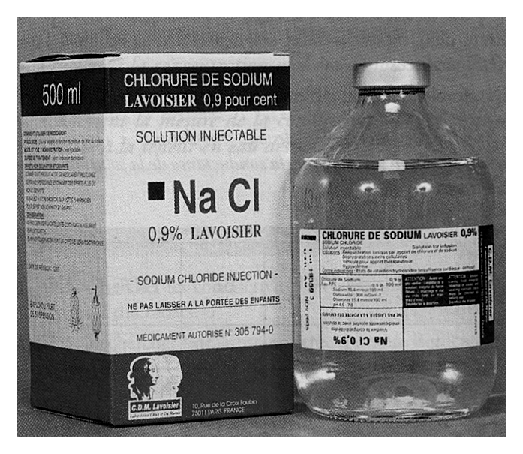
\includegraphics[width=7cm]{tp_prem_s_chimie/tp6_determination_par_conductimetrie_concentration/solution_nacl.png.eps}
\caption{Solution de chlorure de sodium}
\end{figure}
\end{center}


%\end{multicols}


\vressort{3}

\tp{D�termination par conductim�trie\\
de la concentration en solut�\\
d'une solution ionique}


\begin{multicols}{2}

\objectifs{
\item r�aliser une courbe d'�talonnage $G = f(C)$ et en d�duire une
  concentration inconnue.
\item Aborder une limite de la m�thode d'�talonnage.
}
\vspace*{2cm}


\materiel{
\item b�cher $600~mL$
\item fiole jaug�e $500~mL$
\item burette gradu�e $25~mL$
\item pipette jaug�e $5~mL$
\item agitateur magn�tique.
\item solution de chlorure de sodium $S_0$ de concentration $C_0 =
  0,10~mol.L^{-1}$
\item flacon de s�rum physiologique
\item eau d�min�ralis�e
\item g�n�rateur basse fr�quence.
\item 2 multim�tres
\item cellule de conductim�trie.
}


\end{multicols}




\section{R�alisation d'une �chelle de conductance}


\begin{multicols}{2}

\subsection{Protocole op�ratoire}
\begin{enumerate}
\item Rincer la burette, la remplir � l'aide de la solution $S_0$ ajuster le
z�ro.

\item Avec la fiole jaug�e, introduire $V = 500~mL$ d'eau d�min�ralis�e dans
le b�cher.

\item Placer la cellule conductim�trique dans le b�cher et r�aliser le
montage �lectrique correspondant au sch�ma ci-contre. Les 2
multim�tres sont en mode alternatif ($AC$ ou \acsymbol).

\item Sur le GBF, r�gler la fr�quence $500~Hz$ et fixer la tension �
$1,00~V$.

\item Au contenu du b�cher, ajouter les volumes $V_0$ suivants de solution
de chlorure de sodium mesur�s pr�cis�ment gr�ce � la burette. Apr�s
chaque addition, v�rifier que la tension est toujours de $1,00~V$ et
relever la valeur de l'intensit�.

\end{enumerate}




\begin{center}
\begin{figure}[H]
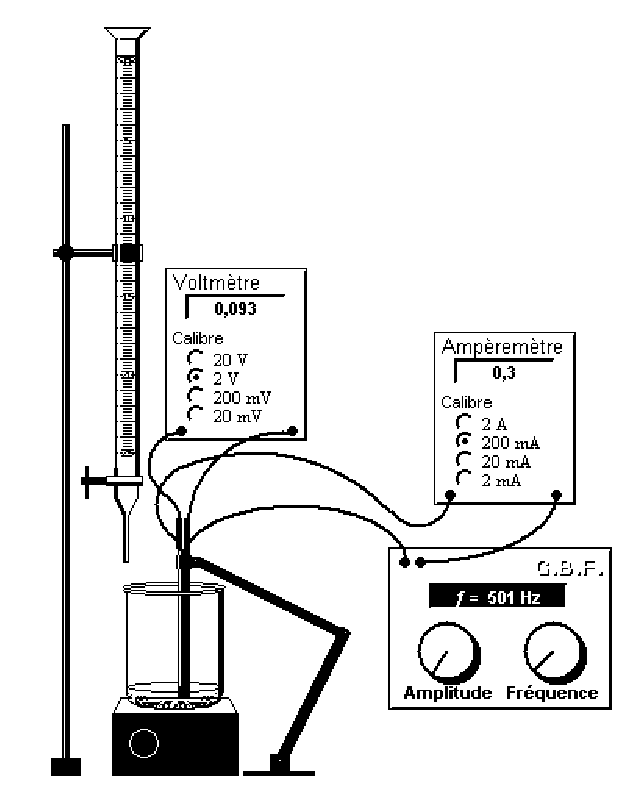
\includegraphics[width=6cm]{tp_prem_s_chimie/tp6_determination_par_conductimetrie_concentration/montage_conductimetrie.png.eps}
\caption{Dispositif exp�rimental}
\end{figure}
\end{center}


\end{multicols}



\subsection{R�sultats}
\begin{enumerate}
\item Calculer la conductance $G$ et compl�ter le tableau suivant.

\begin{arraydata}{6}
\hline
$V_0$ ($mL$)       &  0 &  5 & 10 & 15 & 20 & 25 \\ \hline
\rule[-0.4cm]{0cm}{1cm}
$C$ ($mol.L^{-1}$) &    &    &    &    &    &    \\ \hline
\rule[-0.4cm]{0cm}{1cm}
$G$ ($mS$)         &    &    &    &    &    &    \\ \hline
\end{arraydata}

\item Tracer la courbe d'�talonnage $G = f (C)$.
\end{enumerate}



\pagebreak
%\newpage


\section{D�termination de la concentration en $NaCl$ d'une solution de
  s�rum physiologique}

L'objectif est de d�terminer la concentration du chlorure de sodium dans le s�rum physiologique injectable.

\begin{enumerate}
\item Diluer au $1/100\ieme$ le s�rum physiologique. En pr�parer $500~mL$.

\item D�crire � l'aide de sch�mas le protocole utilis� pour r�aliser
  cette dilution au $1/100\ieme$ et obtenir la solution $S'$.

\item D�terminer la conductance $G'$ de cette solution $S'$.

\item En d�duire la concentration $C'$ du chlorure de sodium dans le
  s�rum physiologique dilu�.

\end{enumerate}


\vressort{3}

\section{Questions compl�mentaires}

%\begin{multicols}{2}

\begin{enumerate}
\item Expliquer comment calculer la concentration $C$ des diff�rentes
  solutions de chlorure de sodium. Donner l'expression de $C$ en
  fonction de $C_0$, $V_0$, $V$.


\item Comment calcule-t-on la conductance $G$ ?

\item Pour quelle raison pratique a-t-on int�r�t � prendre $U =
  1,00~V$ dans les diff�rentes manipulations ?

\item En extrapolant la courbe d'�talonnage, pr�voir la conductance
  d'une portion de solution concentr�e � $T = 58,4~g.L^{-1}$. Mesurer
  la conductance r�elle d'une portion d'une telle solution. Que
  peut-on conclure quant � la m�thode d'�talonnage utilis�e. On donne
  $M_{Na} = 23~g.mol^{-1}$ et $M_{Cl} = 35,5~g.mol^{-1}$.

\item Rappeler la valeur de la concentration $C'$ du chlorure de
  sodium dans le s�rum physiologique dilu�.

\item Comment peut-on alors d�terminer la concentration $C_0'$ du
  chlorure de sodium dans la solution commerciale de s�rum
  physiologique ? Calculer cette concentration $C_0'$ puis le titre
  massique (concentration massique) correspondant $T_0$. Le comparer avec
  les indications figurant sur l'�tiquette du flacon ($0,9~\%$ en masse).
\end{enumerate}


%\vressort{1}
\vressort{3}

\begin{center}
\begin{figure}[H]
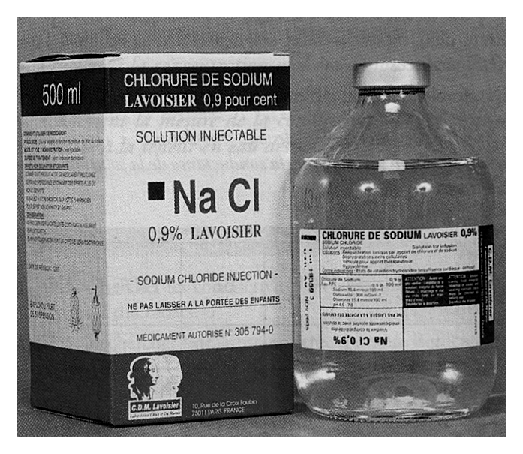
\includegraphics[width=7cm]{tp_prem_s_chimie/tp6_determination_par_conductimetrie_concentration/solution_nacl.png.eps}
\caption{Solution de chlorure de sodium}
\end{figure}
\end{center}


%\end{multicols}


\vressort{3}
\tp{D�termination par conductim�trie\\
de la concentration en solut�\\
d'une solution ionique}


\begin{multicols}{2}

\objectifs{
\item r�aliser une courbe d'�talonnage $G = f(C)$ et en d�duire une
  concentration inconnue.
\item Aborder une limite de la m�thode d'�talonnage.
}
\vspace*{2cm}


\materiel{
\item b�cher $600~mL$
\item fiole jaug�e $500~mL$
\item burette gradu�e $25~mL$
\item pipette jaug�e $5~mL$
\item agitateur magn�tique.
\item solution de chlorure de sodium $S_0$ de concentration $C_0 =
  0,10~mol.L^{-1}$
\item flacon de s�rum physiologique
\item eau d�min�ralis�e
\item g�n�rateur basse fr�quence.
\item 2 multim�tres
\item cellule de conductim�trie.
}


\end{multicols}




\section{R�alisation d'une �chelle de conductance}


\begin{multicols}{2}

\subsection{Protocole op�ratoire}
\begin{enumerate}
\item Rincer la burette, la remplir � l'aide de la solution $S_0$ ajuster le
z�ro.

\item Avec la fiole jaug�e, introduire $V = 500~mL$ d'eau d�min�ralis�e dans
le b�cher.

\item Placer la cellule conductim�trique dans le b�cher et r�aliser le
montage �lectrique correspondant au sch�ma ci-contre. Les 2
multim�tres sont en mode alternatif ($AC$ ou \acsymbol).

\item Sur le GBF, r�gler la fr�quence $500~Hz$ et fixer la tension �
$1,00~V$.

\item Au contenu du b�cher, ajouter les volumes $V_0$ suivants de solution
de chlorure de sodium mesur�s pr�cis�ment gr�ce � la burette. Apr�s
chaque addition, v�rifier que la tension est toujours de $1,00~V$ et
relever la valeur de l'intensit�.

\end{enumerate}




\begin{center}
\begin{figure}[H]
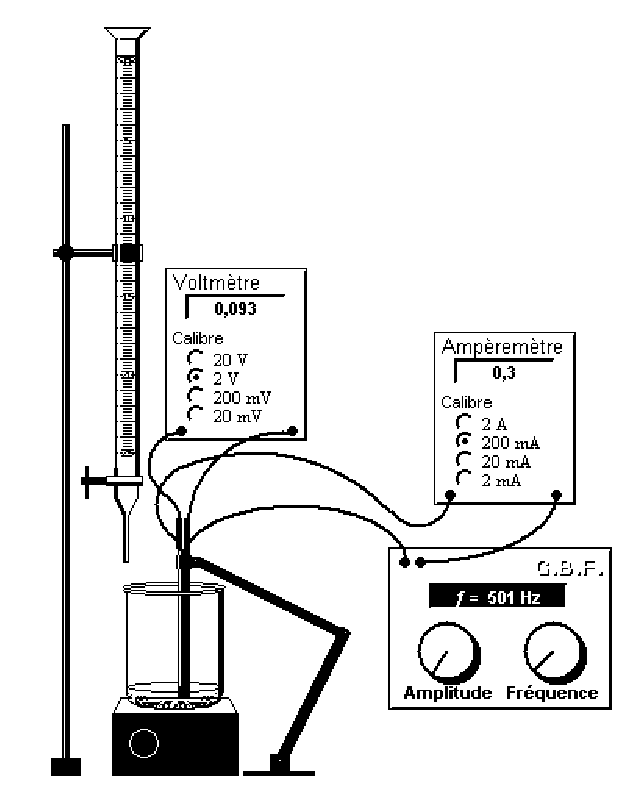
\includegraphics[width=6cm]{tp_prem_s_chimie/tp6_determination_par_conductimetrie_concentration/montage_conductimetrie.png.eps}
\caption{Dispositif exp�rimental}
\end{figure}
\end{center}


\end{multicols}



\subsection{R�sultats}
\begin{enumerate}
\item Calculer la conductance $G$ et compl�ter le tableau suivant.

\begin{arraydata}{6}
\hline
$V_0$ ($mL$)       &  0 &  5 & 10 & 15 & 20 & 25 \\ \hline
\rule[-0.4cm]{0cm}{1cm}
$C$ ($mol.L^{-1}$) &    &    &    &    &    &    \\ \hline
\rule[-0.4cm]{0cm}{1cm}
$G$ ($mS$)         &    &    &    &    &    &    \\ \hline
\end{arraydata}

\item Tracer la courbe d'�talonnage $G = f (C)$.
\end{enumerate}



\pagebreak
%\newpage


\section{D�termination de la concentration en $NaCl$ d'une solution de
  s�rum physiologique}

L'objectif est de d�terminer la concentration du chlorure de sodium dans le s�rum physiologique injectable.

\begin{enumerate}
\item Diluer au $1/100\ieme$ le s�rum physiologique. En pr�parer $500~mL$.

\item D�crire � l'aide de sch�mas le protocole utilis� pour r�aliser
  cette dilution au $1/100\ieme$ et obtenir la solution $S'$.

\item D�terminer la conductance $G'$ de cette solution $S'$.

\item En d�duire la concentration $C'$ du chlorure de sodium dans le
  s�rum physiologique dilu�.

\end{enumerate}


\vressort{3}

\section{Questions compl�mentaires}

%\begin{multicols}{2}

\begin{enumerate}
\item Expliquer comment calculer la concentration $C$ des diff�rentes
  solutions de chlorure de sodium. Donner l'expression de $C$ en
  fonction de $C_0$, $V_0$, $V$.


\item Comment calcule-t-on la conductance $G$ ?

\item Pour quelle raison pratique a-t-on int�r�t � prendre $U =
  1,00~V$ dans les diff�rentes manipulations ?

\item En extrapolant la courbe d'�talonnage, pr�voir la conductance
  d'une portion de solution concentr�e � $T = 58,4~g.L^{-1}$. Mesurer
  la conductance r�elle d'une portion d'une telle solution. Que
  peut-on conclure quant � la m�thode d'�talonnage utilis�e. On donne
  $M_{Na} = 23~g.mol^{-1}$ et $M_{Cl} = 35,5~g.mol^{-1}$.

\item Rappeler la valeur de la concentration $C'$ du chlorure de
  sodium dans le s�rum physiologique dilu�.

\item Comment peut-on alors d�terminer la concentration $C_0'$ du
  chlorure de sodium dans la solution commerciale de s�rum
  physiologique ? Calculer cette concentration $C_0'$ puis le titre
  massique (concentration massique) correspondant $T_0$. Le comparer avec
  les indications figurant sur l'�tiquette du flacon ($0,9~\%$ en masse).
\end{enumerate}


%\vressort{1}
\vressort{3}

\begin{center}
\begin{figure}[H]
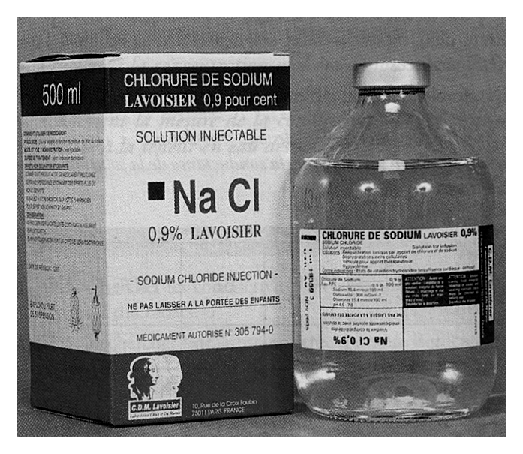
\includegraphics[width=7cm]{tp_prem_s_chimie/tp6_determination_par_conductimetrie_concentration/solution_nacl.png.eps}
\caption{Solution de chlorure de sodium}
\end{figure}
\end{center}


%\end{multicols}


\vressort{3}
\tp{D�termination par conductim�trie\\
de la concentration en solut�\\
d'une solution ionique}


\begin{multicols}{2}

\objectifs{
\item r�aliser une courbe d'�talonnage $G = f(C)$ et en d�duire une
  concentration inconnue.
\item Aborder une limite de la m�thode d'�talonnage.
}
\vspace*{2cm}


\materiel{
\item b�cher $600~mL$
\item fiole jaug�e $500~mL$
\item burette gradu�e $25~mL$
\item pipette jaug�e $5~mL$
\item agitateur magn�tique.
\item solution de chlorure de sodium $S_0$ de concentration $C_0 =
  0,10~mol.L^{-1}$
\item flacon de s�rum physiologique
\item eau d�min�ralis�e
\item g�n�rateur basse fr�quence.
\item 2 multim�tres
\item cellule de conductim�trie.
}


\end{multicols}




\section{R�alisation d'une �chelle de conductance}


\begin{multicols}{2}

\subsection{Protocole op�ratoire}
\begin{enumerate}
\item Rincer la burette, la remplir � l'aide de la solution $S_0$ ajuster le
z�ro.

\item Avec la fiole jaug�e, introduire $V = 500~mL$ d'eau d�min�ralis�e dans
le b�cher.

\item Placer la cellule conductim�trique dans le b�cher et r�aliser le
montage �lectrique correspondant au sch�ma ci-contre. Les 2
multim�tres sont en mode alternatif ($AC$ ou \acsymbol).

\item Sur le GBF, r�gler la fr�quence $500~Hz$ et fixer la tension �
$1,00~V$.

\item Au contenu du b�cher, ajouter les volumes $V_0$ suivants de solution
de chlorure de sodium mesur�s pr�cis�ment gr�ce � la burette. Apr�s
chaque addition, v�rifier que la tension est toujours de $1,00~V$ et
relever la valeur de l'intensit�.

\end{enumerate}




\begin{center}
\begin{figure}[H]
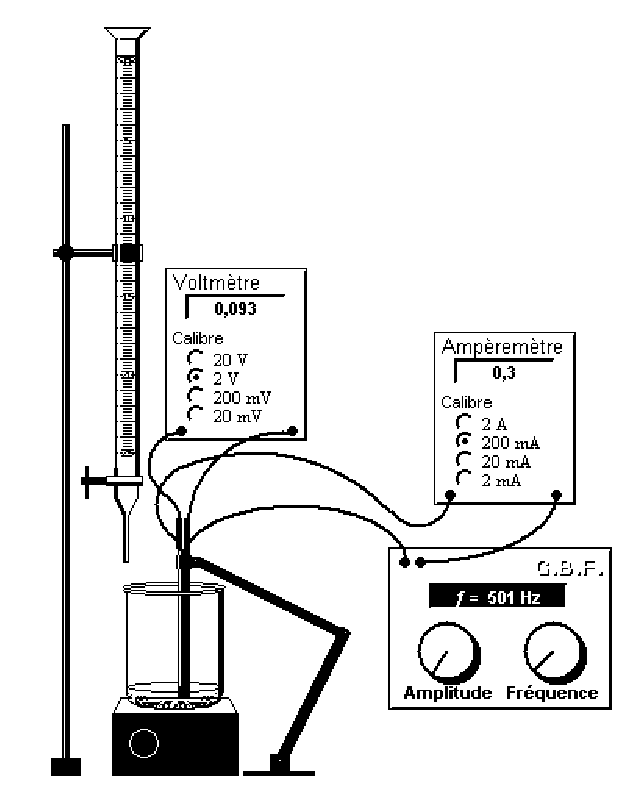
\includegraphics[width=6cm]{tp_prem_s_chimie/tp6_determination_par_conductimetrie_concentration/montage_conductimetrie.png.eps}
\caption{Dispositif exp�rimental}
\end{figure}
\end{center}


\end{multicols}



\subsection{R�sultats}
\begin{enumerate}
\item Calculer la conductance $G$ et compl�ter le tableau suivant.

\begin{arraydata}{6}
\hline
$V_0$ ($mL$)       &  0 &  5 & 10 & 15 & 20 & 25 \\ \hline
\rule[-0.4cm]{0cm}{1cm}
$C$ ($mol.L^{-1}$) &    &    &    &    &    &    \\ \hline
\rule[-0.4cm]{0cm}{1cm}
$G$ ($mS$)         &    &    &    &    &    &    \\ \hline
\end{arraydata}

\item Tracer la courbe d'�talonnage $G = f (C)$.
\end{enumerate}



\pagebreak
%\newpage


\section{D�termination de la concentration en $NaCl$ d'une solution de
  s�rum physiologique}

L'objectif est de d�terminer la concentration du chlorure de sodium dans le s�rum physiologique injectable.

\begin{enumerate}
\item Diluer au $1/100\ieme$ le s�rum physiologique. En pr�parer $500~mL$.

\item D�crire � l'aide de sch�mas le protocole utilis� pour r�aliser
  cette dilution au $1/100\ieme$ et obtenir la solution $S'$.

\item D�terminer la conductance $G'$ de cette solution $S'$.

\item En d�duire la concentration $C'$ du chlorure de sodium dans le
  s�rum physiologique dilu�.

\end{enumerate}


\vressort{3}

\section{Questions compl�mentaires}

%\begin{multicols}{2}

\begin{enumerate}
\item Expliquer comment calculer la concentration $C$ des diff�rentes
  solutions de chlorure de sodium. Donner l'expression de $C$ en
  fonction de $C_0$, $V_0$, $V$.


\item Comment calcule-t-on la conductance $G$ ?

\item Pour quelle raison pratique a-t-on int�r�t � prendre $U =
  1,00~V$ dans les diff�rentes manipulations ?

\item En extrapolant la courbe d'�talonnage, pr�voir la conductance
  d'une portion de solution concentr�e � $T = 58,4~g.L^{-1}$. Mesurer
  la conductance r�elle d'une portion d'une telle solution. Que
  peut-on conclure quant � la m�thode d'�talonnage utilis�e. On donne
  $M_{Na} = 23~g.mol^{-1}$ et $M_{Cl} = 35,5~g.mol^{-1}$.

\item Rappeler la valeur de la concentration $C'$ du chlorure de
  sodium dans le s�rum physiologique dilu�.

\item Comment peut-on alors d�terminer la concentration $C_0'$ du
  chlorure de sodium dans la solution commerciale de s�rum
  physiologique ? Calculer cette concentration $C_0'$ puis le titre
  massique (concentration massique) correspondant $T_0$. Le comparer avec
  les indications figurant sur l'�tiquette du flacon ($0,9~\%$ en masse).
\end{enumerate}


%\vressort{1}
\vressort{3}

\begin{center}
\begin{figure}[H]
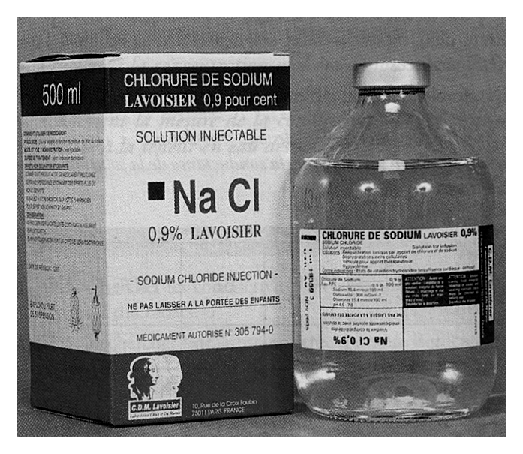
\includegraphics[width=7cm]{tp_prem_s_chimie/tp6_determination_par_conductimetrie_concentration/solution_nacl.png.eps}
\caption{Solution de chlorure de sodium}
\end{figure}
\end{center}


%\end{multicols}


\vressort{3} % Lentilles (Images, rel
                                % de conjugaison)
\tp{D�termination par conductim�trie\\
de la concentration en solut�\\
d'une solution ionique}


\begin{multicols}{2}

\objectifs{
\item r�aliser une courbe d'�talonnage $G = f(C)$ et en d�duire une
  concentration inconnue.
\item Aborder une limite de la m�thode d'�talonnage.
}
\vspace*{2cm}


\materiel{
\item b�cher $600~mL$
\item fiole jaug�e $500~mL$
\item burette gradu�e $25~mL$
\item pipette jaug�e $5~mL$
\item agitateur magn�tique.
\item solution de chlorure de sodium $S_0$ de concentration $C_0 =
  0,10~mol.L^{-1}$
\item flacon de s�rum physiologique
\item eau d�min�ralis�e
\item g�n�rateur basse fr�quence.
\item 2 multim�tres
\item cellule de conductim�trie.
}


\end{multicols}




\section{R�alisation d'une �chelle de conductance}


\begin{multicols}{2}

\subsection{Protocole op�ratoire}
\begin{enumerate}
\item Rincer la burette, la remplir � l'aide de la solution $S_0$ ajuster le
z�ro.

\item Avec la fiole jaug�e, introduire $V = 500~mL$ d'eau d�min�ralis�e dans
le b�cher.

\item Placer la cellule conductim�trique dans le b�cher et r�aliser le
montage �lectrique correspondant au sch�ma ci-contre. Les 2
multim�tres sont en mode alternatif ($AC$ ou \acsymbol).

\item Sur le GBF, r�gler la fr�quence $500~Hz$ et fixer la tension �
$1,00~V$.

\item Au contenu du b�cher, ajouter les volumes $V_0$ suivants de solution
de chlorure de sodium mesur�s pr�cis�ment gr�ce � la burette. Apr�s
chaque addition, v�rifier que la tension est toujours de $1,00~V$ et
relever la valeur de l'intensit�.

\end{enumerate}




\begin{center}
\begin{figure}[H]
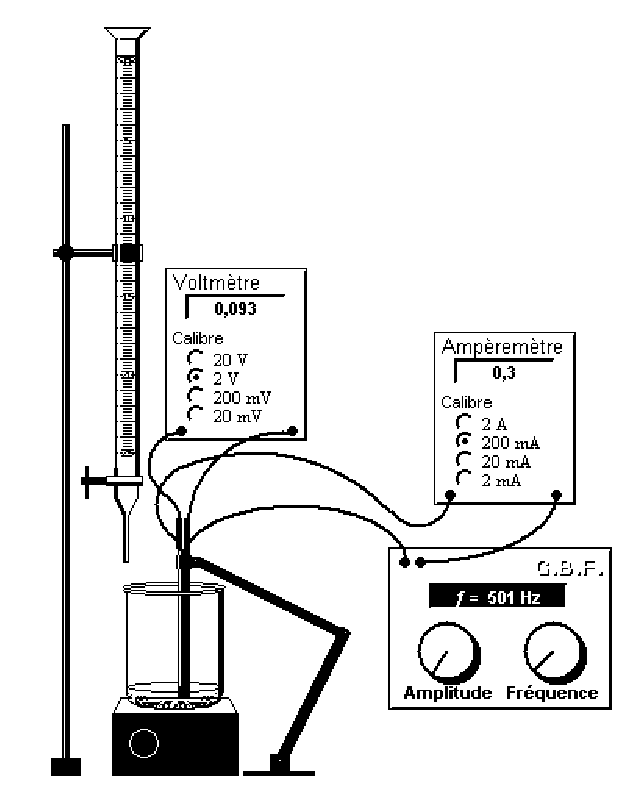
\includegraphics[width=6cm]{tp_prem_s_chimie/tp6_determination_par_conductimetrie_concentration/montage_conductimetrie.png.eps}
\caption{Dispositif exp�rimental}
\end{figure}
\end{center}


\end{multicols}



\subsection{R�sultats}
\begin{enumerate}
\item Calculer la conductance $G$ et compl�ter le tableau suivant.

\begin{arraydata}{6}
\hline
$V_0$ ($mL$)       &  0 &  5 & 10 & 15 & 20 & 25 \\ \hline
\rule[-0.4cm]{0cm}{1cm}
$C$ ($mol.L^{-1}$) &    &    &    &    &    &    \\ \hline
\rule[-0.4cm]{0cm}{1cm}
$G$ ($mS$)         &    &    &    &    &    &    \\ \hline
\end{arraydata}

\item Tracer la courbe d'�talonnage $G = f (C)$.
\end{enumerate}



\pagebreak
%\newpage


\section{D�termination de la concentration en $NaCl$ d'une solution de
  s�rum physiologique}

L'objectif est de d�terminer la concentration du chlorure de sodium dans le s�rum physiologique injectable.

\begin{enumerate}
\item Diluer au $1/100\ieme$ le s�rum physiologique. En pr�parer $500~mL$.

\item D�crire � l'aide de sch�mas le protocole utilis� pour r�aliser
  cette dilution au $1/100\ieme$ et obtenir la solution $S'$.

\item D�terminer la conductance $G'$ de cette solution $S'$.

\item En d�duire la concentration $C'$ du chlorure de sodium dans le
  s�rum physiologique dilu�.

\end{enumerate}


\vressort{3}

\section{Questions compl�mentaires}

%\begin{multicols}{2}

\begin{enumerate}
\item Expliquer comment calculer la concentration $C$ des diff�rentes
  solutions de chlorure de sodium. Donner l'expression de $C$ en
  fonction de $C_0$, $V_0$, $V$.


\item Comment calcule-t-on la conductance $G$ ?

\item Pour quelle raison pratique a-t-on int�r�t � prendre $U =
  1,00~V$ dans les diff�rentes manipulations ?

\item En extrapolant la courbe d'�talonnage, pr�voir la conductance
  d'une portion de solution concentr�e � $T = 58,4~g.L^{-1}$. Mesurer
  la conductance r�elle d'une portion d'une telle solution. Que
  peut-on conclure quant � la m�thode d'�talonnage utilis�e. On donne
  $M_{Na} = 23~g.mol^{-1}$ et $M_{Cl} = 35,5~g.mol^{-1}$.

\item Rappeler la valeur de la concentration $C'$ du chlorure de
  sodium dans le s�rum physiologique dilu�.

\item Comment peut-on alors d�terminer la concentration $C_0'$ du
  chlorure de sodium dans la solution commerciale de s�rum
  physiologique ? Calculer cette concentration $C_0'$ puis le titre
  massique (concentration massique) correspondant $T_0$. Le comparer avec
  les indications figurant sur l'�tiquette du flacon ($0,9~\%$ en masse).
\end{enumerate}


%\vressort{1}
\vressort{3}

\begin{center}
\begin{figure}[H]
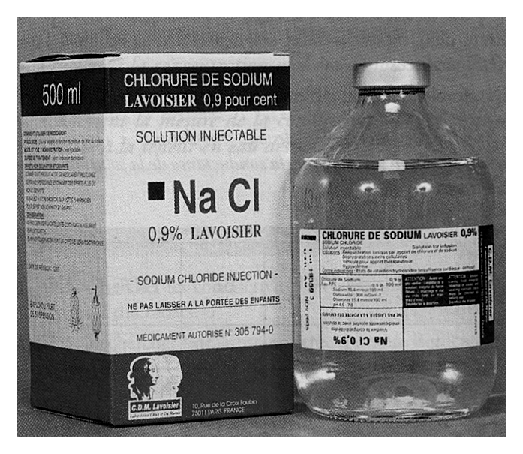
\includegraphics[width=7cm]{tp_prem_s_chimie/tp6_determination_par_conductimetrie_concentration/solution_nacl.png.eps}
\caption{Solution de chlorure de sodium}
\end{figure}
\end{center}


%\end{multicols}


\vressort{3}

\tp{D�termination par conductim�trie\\
de la concentration en solut�\\
d'une solution ionique}


\begin{multicols}{2}

\objectifs{
\item r�aliser une courbe d'�talonnage $G = f(C)$ et en d�duire une
  concentration inconnue.
\item Aborder une limite de la m�thode d'�talonnage.
}
\vspace*{2cm}


\materiel{
\item b�cher $600~mL$
\item fiole jaug�e $500~mL$
\item burette gradu�e $25~mL$
\item pipette jaug�e $5~mL$
\item agitateur magn�tique.
\item solution de chlorure de sodium $S_0$ de concentration $C_0 =
  0,10~mol.L^{-1}$
\item flacon de s�rum physiologique
\item eau d�min�ralis�e
\item g�n�rateur basse fr�quence.
\item 2 multim�tres
\item cellule de conductim�trie.
}


\end{multicols}




\section{R�alisation d'une �chelle de conductance}


\begin{multicols}{2}

\subsection{Protocole op�ratoire}
\begin{enumerate}
\item Rincer la burette, la remplir � l'aide de la solution $S_0$ ajuster le
z�ro.

\item Avec la fiole jaug�e, introduire $V = 500~mL$ d'eau d�min�ralis�e dans
le b�cher.

\item Placer la cellule conductim�trique dans le b�cher et r�aliser le
montage �lectrique correspondant au sch�ma ci-contre. Les 2
multim�tres sont en mode alternatif ($AC$ ou \acsymbol).

\item Sur le GBF, r�gler la fr�quence $500~Hz$ et fixer la tension �
$1,00~V$.

\item Au contenu du b�cher, ajouter les volumes $V_0$ suivants de solution
de chlorure de sodium mesur�s pr�cis�ment gr�ce � la burette. Apr�s
chaque addition, v�rifier que la tension est toujours de $1,00~V$ et
relever la valeur de l'intensit�.

\end{enumerate}




\begin{center}
\begin{figure}[H]
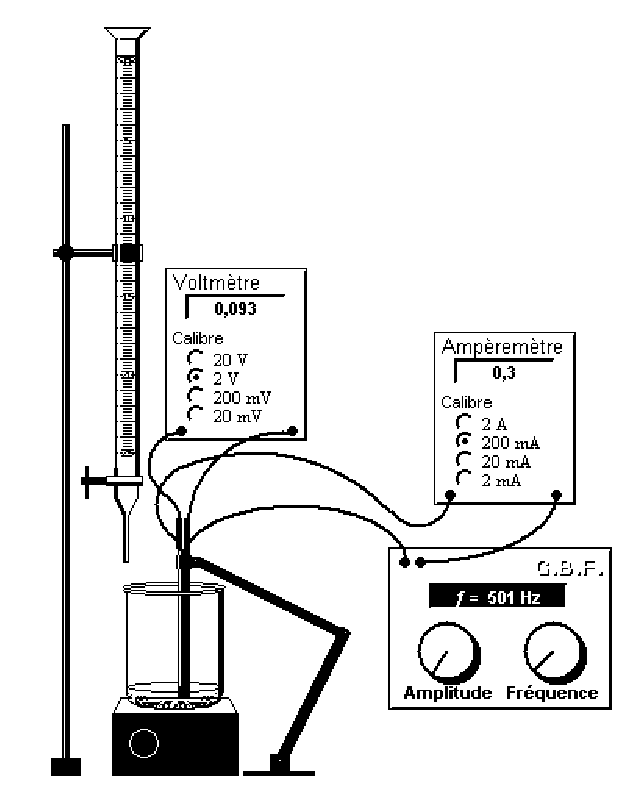
\includegraphics[width=6cm]{tp_prem_s_chimie/tp6_determination_par_conductimetrie_concentration/montage_conductimetrie.png.eps}
\caption{Dispositif exp�rimental}
\end{figure}
\end{center}


\end{multicols}



\subsection{R�sultats}
\begin{enumerate}
\item Calculer la conductance $G$ et compl�ter le tableau suivant.

\begin{arraydata}{6}
\hline
$V_0$ ($mL$)       &  0 &  5 & 10 & 15 & 20 & 25 \\ \hline
\rule[-0.4cm]{0cm}{1cm}
$C$ ($mol.L^{-1}$) &    &    &    &    &    &    \\ \hline
\rule[-0.4cm]{0cm}{1cm}
$G$ ($mS$)         &    &    &    &    &    &    \\ \hline
\end{arraydata}

\item Tracer la courbe d'�talonnage $G = f (C)$.
\end{enumerate}



\pagebreak
%\newpage


\section{D�termination de la concentration en $NaCl$ d'une solution de
  s�rum physiologique}

L'objectif est de d�terminer la concentration du chlorure de sodium dans le s�rum physiologique injectable.

\begin{enumerate}
\item Diluer au $1/100\ieme$ le s�rum physiologique. En pr�parer $500~mL$.

\item D�crire � l'aide de sch�mas le protocole utilis� pour r�aliser
  cette dilution au $1/100\ieme$ et obtenir la solution $S'$.

\item D�terminer la conductance $G'$ de cette solution $S'$.

\item En d�duire la concentration $C'$ du chlorure de sodium dans le
  s�rum physiologique dilu�.

\end{enumerate}


\vressort{3}

\section{Questions compl�mentaires}

%\begin{multicols}{2}

\begin{enumerate}
\item Expliquer comment calculer la concentration $C$ des diff�rentes
  solutions de chlorure de sodium. Donner l'expression de $C$ en
  fonction de $C_0$, $V_0$, $V$.


\item Comment calcule-t-on la conductance $G$ ?

\item Pour quelle raison pratique a-t-on int�r�t � prendre $U =
  1,00~V$ dans les diff�rentes manipulations ?

\item En extrapolant la courbe d'�talonnage, pr�voir la conductance
  d'une portion de solution concentr�e � $T = 58,4~g.L^{-1}$. Mesurer
  la conductance r�elle d'une portion d'une telle solution. Que
  peut-on conclure quant � la m�thode d'�talonnage utilis�e. On donne
  $M_{Na} = 23~g.mol^{-1}$ et $M_{Cl} = 35,5~g.mol^{-1}$.

\item Rappeler la valeur de la concentration $C'$ du chlorure de
  sodium dans le s�rum physiologique dilu�.

\item Comment peut-on alors d�terminer la concentration $C_0'$ du
  chlorure de sodium dans la solution commerciale de s�rum
  physiologique ? Calculer cette concentration $C_0'$ puis le titre
  massique (concentration massique) correspondant $T_0$. Le comparer avec
  les indications figurant sur l'�tiquette du flacon ($0,9~\%$ en masse).
\end{enumerate}


%\vressort{1}
\vressort{3}

\begin{center}
\begin{figure}[H]
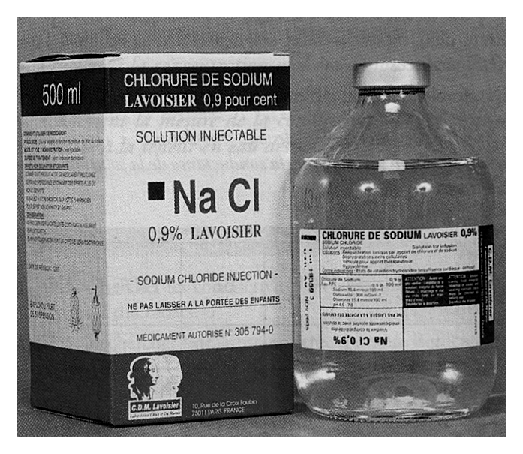
\includegraphics[width=7cm]{tp_prem_s_chimie/tp6_determination_par_conductimetrie_concentration/solution_nacl.png.eps}
\caption{Solution de chlorure de sodium}
\end{figure}
\end{center}


%\end{multicols}


\vressort{3} % Focom�trie lentilles
                                % minces

% lunette astronomique





\chapitre{M�canique}
\tp{D�termination par conductim�trie\\
de la concentration en solut�\\
d'une solution ionique}


\begin{multicols}{2}

\objectifs{
\item r�aliser une courbe d'�talonnage $G = f(C)$ et en d�duire une
  concentration inconnue.
\item Aborder une limite de la m�thode d'�talonnage.
}
\vspace*{2cm}


\materiel{
\item b�cher $600~mL$
\item fiole jaug�e $500~mL$
\item burette gradu�e $25~mL$
\item pipette jaug�e $5~mL$
\item agitateur magn�tique.
\item solution de chlorure de sodium $S_0$ de concentration $C_0 =
  0,10~mol.L^{-1}$
\item flacon de s�rum physiologique
\item eau d�min�ralis�e
\item g�n�rateur basse fr�quence.
\item 2 multim�tres
\item cellule de conductim�trie.
}


\end{multicols}




\section{R�alisation d'une �chelle de conductance}


\begin{multicols}{2}

\subsection{Protocole op�ratoire}
\begin{enumerate}
\item Rincer la burette, la remplir � l'aide de la solution $S_0$ ajuster le
z�ro.

\item Avec la fiole jaug�e, introduire $V = 500~mL$ d'eau d�min�ralis�e dans
le b�cher.

\item Placer la cellule conductim�trique dans le b�cher et r�aliser le
montage �lectrique correspondant au sch�ma ci-contre. Les 2
multim�tres sont en mode alternatif ($AC$ ou \acsymbol).

\item Sur le GBF, r�gler la fr�quence $500~Hz$ et fixer la tension �
$1,00~V$.

\item Au contenu du b�cher, ajouter les volumes $V_0$ suivants de solution
de chlorure de sodium mesur�s pr�cis�ment gr�ce � la burette. Apr�s
chaque addition, v�rifier que la tension est toujours de $1,00~V$ et
relever la valeur de l'intensit�.

\end{enumerate}




\begin{center}
\begin{figure}[H]
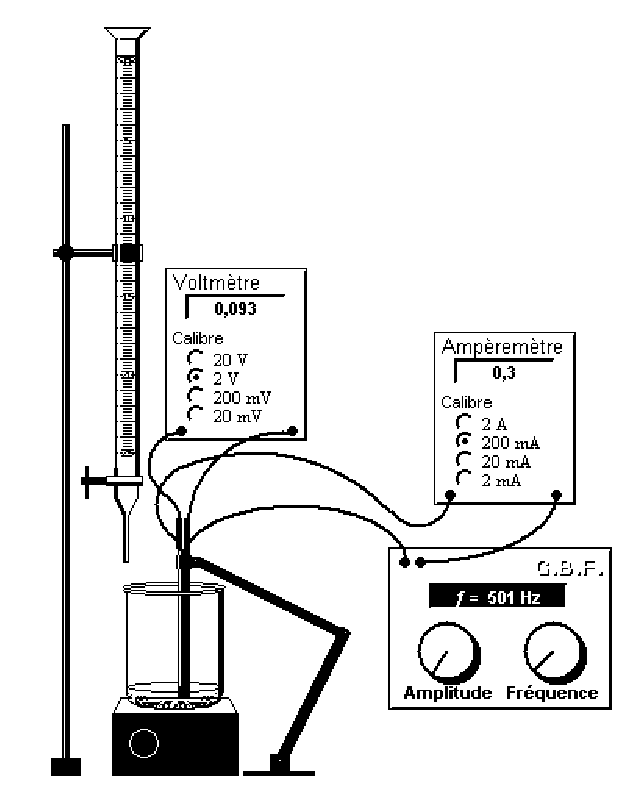
\includegraphics[width=6cm]{tp_prem_s_chimie/tp6_determination_par_conductimetrie_concentration/montage_conductimetrie.png.eps}
\caption{Dispositif exp�rimental}
\end{figure}
\end{center}


\end{multicols}



\subsection{R�sultats}
\begin{enumerate}
\item Calculer la conductance $G$ et compl�ter le tableau suivant.

\begin{arraydata}{6}
\hline
$V_0$ ($mL$)       &  0 &  5 & 10 & 15 & 20 & 25 \\ \hline
\rule[-0.4cm]{0cm}{1cm}
$C$ ($mol.L^{-1}$) &    &    &    &    &    &    \\ \hline
\rule[-0.4cm]{0cm}{1cm}
$G$ ($mS$)         &    &    &    &    &    &    \\ \hline
\end{arraydata}

\item Tracer la courbe d'�talonnage $G = f (C)$.
\end{enumerate}



\pagebreak
%\newpage


\section{D�termination de la concentration en $NaCl$ d'une solution de
  s�rum physiologique}

L'objectif est de d�terminer la concentration du chlorure de sodium dans le s�rum physiologique injectable.

\begin{enumerate}
\item Diluer au $1/100\ieme$ le s�rum physiologique. En pr�parer $500~mL$.

\item D�crire � l'aide de sch�mas le protocole utilis� pour r�aliser
  cette dilution au $1/100\ieme$ et obtenir la solution $S'$.

\item D�terminer la conductance $G'$ de cette solution $S'$.

\item En d�duire la concentration $C'$ du chlorure de sodium dans le
  s�rum physiologique dilu�.

\end{enumerate}


\vressort{3}

\section{Questions compl�mentaires}

%\begin{multicols}{2}

\begin{enumerate}
\item Expliquer comment calculer la concentration $C$ des diff�rentes
  solutions de chlorure de sodium. Donner l'expression de $C$ en
  fonction de $C_0$, $V_0$, $V$.


\item Comment calcule-t-on la conductance $G$ ?

\item Pour quelle raison pratique a-t-on int�r�t � prendre $U =
  1,00~V$ dans les diff�rentes manipulations ?

\item En extrapolant la courbe d'�talonnage, pr�voir la conductance
  d'une portion de solution concentr�e � $T = 58,4~g.L^{-1}$. Mesurer
  la conductance r�elle d'une portion d'une telle solution. Que
  peut-on conclure quant � la m�thode d'�talonnage utilis�e. On donne
  $M_{Na} = 23~g.mol^{-1}$ et $M_{Cl} = 35,5~g.mol^{-1}$.

\item Rappeler la valeur de la concentration $C'$ du chlorure de
  sodium dans le s�rum physiologique dilu�.

\item Comment peut-on alors d�terminer la concentration $C_0'$ du
  chlorure de sodium dans la solution commerciale de s�rum
  physiologique ? Calculer cette concentration $C_0'$ puis le titre
  massique (concentration massique) correspondant $T_0$. Le comparer avec
  les indications figurant sur l'�tiquette du flacon ($0,9~\%$ en masse).
\end{enumerate}


%\vressort{1}
\vressort{3}

\begin{center}
\begin{figure}[H]
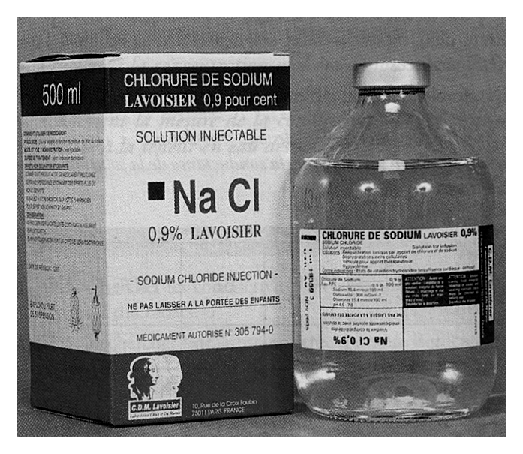
\includegraphics[width=7cm]{tp_prem_s_chimie/tp6_determination_par_conductimetrie_concentration/solution_nacl.png.eps}
\caption{Solution de chlorure de sodium}
\end{figure}
\end{center}


%\end{multicols}


\vressort{3}


\tp{D�termination par conductim�trie\\
de la concentration en solut�\\
d'une solution ionique}


\begin{multicols}{2}

\objectifs{
\item r�aliser une courbe d'�talonnage $G = f(C)$ et en d�duire une
  concentration inconnue.
\item Aborder une limite de la m�thode d'�talonnage.
}
\vspace*{2cm}


\materiel{
\item b�cher $600~mL$
\item fiole jaug�e $500~mL$
\item burette gradu�e $25~mL$
\item pipette jaug�e $5~mL$
\item agitateur magn�tique.
\item solution de chlorure de sodium $S_0$ de concentration $C_0 =
  0,10~mol.L^{-1}$
\item flacon de s�rum physiologique
\item eau d�min�ralis�e
\item g�n�rateur basse fr�quence.
\item 2 multim�tres
\item cellule de conductim�trie.
}


\end{multicols}




\section{R�alisation d'une �chelle de conductance}


\begin{multicols}{2}

\subsection{Protocole op�ratoire}
\begin{enumerate}
\item Rincer la burette, la remplir � l'aide de la solution $S_0$ ajuster le
z�ro.

\item Avec la fiole jaug�e, introduire $V = 500~mL$ d'eau d�min�ralis�e dans
le b�cher.

\item Placer la cellule conductim�trique dans le b�cher et r�aliser le
montage �lectrique correspondant au sch�ma ci-contre. Les 2
multim�tres sont en mode alternatif ($AC$ ou \acsymbol).

\item Sur le GBF, r�gler la fr�quence $500~Hz$ et fixer la tension �
$1,00~V$.

\item Au contenu du b�cher, ajouter les volumes $V_0$ suivants de solution
de chlorure de sodium mesur�s pr�cis�ment gr�ce � la burette. Apr�s
chaque addition, v�rifier que la tension est toujours de $1,00~V$ et
relever la valeur de l'intensit�.

\end{enumerate}




\begin{center}
\begin{figure}[H]
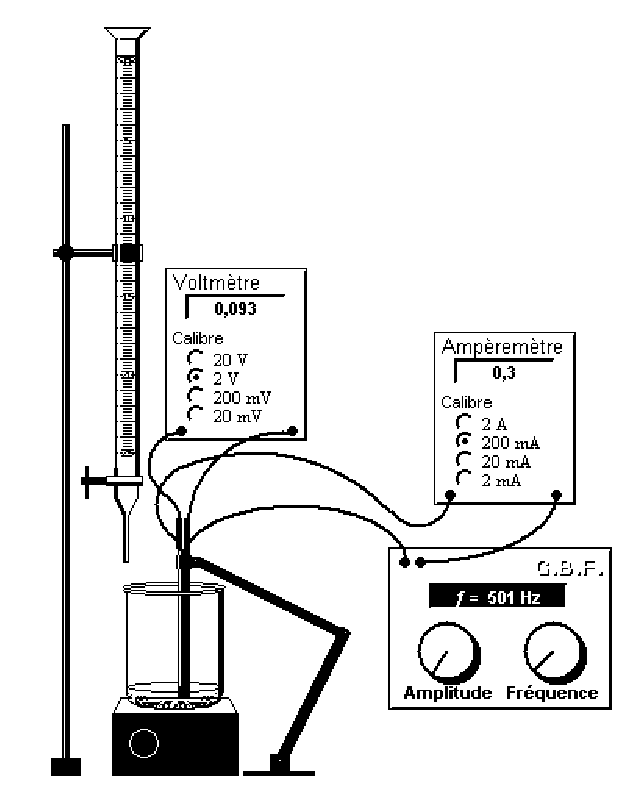
\includegraphics[width=6cm]{tp_prem_s_chimie/tp6_determination_par_conductimetrie_concentration/montage_conductimetrie.png.eps}
\caption{Dispositif exp�rimental}
\end{figure}
\end{center}


\end{multicols}



\subsection{R�sultats}
\begin{enumerate}
\item Calculer la conductance $G$ et compl�ter le tableau suivant.

\begin{arraydata}{6}
\hline
$V_0$ ($mL$)       &  0 &  5 & 10 & 15 & 20 & 25 \\ \hline
\rule[-0.4cm]{0cm}{1cm}
$C$ ($mol.L^{-1}$) &    &    &    &    &    &    \\ \hline
\rule[-0.4cm]{0cm}{1cm}
$G$ ($mS$)         &    &    &    &    &    &    \\ \hline
\end{arraydata}

\item Tracer la courbe d'�talonnage $G = f (C)$.
\end{enumerate}



\pagebreak
%\newpage


\section{D�termination de la concentration en $NaCl$ d'une solution de
  s�rum physiologique}

L'objectif est de d�terminer la concentration du chlorure de sodium dans le s�rum physiologique injectable.

\begin{enumerate}
\item Diluer au $1/100\ieme$ le s�rum physiologique. En pr�parer $500~mL$.

\item D�crire � l'aide de sch�mas le protocole utilis� pour r�aliser
  cette dilution au $1/100\ieme$ et obtenir la solution $S'$.

\item D�terminer la conductance $G'$ de cette solution $S'$.

\item En d�duire la concentration $C'$ du chlorure de sodium dans le
  s�rum physiologique dilu�.

\end{enumerate}


\vressort{3}

\section{Questions compl�mentaires}

%\begin{multicols}{2}

\begin{enumerate}
\item Expliquer comment calculer la concentration $C$ des diff�rentes
  solutions de chlorure de sodium. Donner l'expression de $C$ en
  fonction de $C_0$, $V_0$, $V$.


\item Comment calcule-t-on la conductance $G$ ?

\item Pour quelle raison pratique a-t-on int�r�t � prendre $U =
  1,00~V$ dans les diff�rentes manipulations ?

\item En extrapolant la courbe d'�talonnage, pr�voir la conductance
  d'une portion de solution concentr�e � $T = 58,4~g.L^{-1}$. Mesurer
  la conductance r�elle d'une portion d'une telle solution. Que
  peut-on conclure quant � la m�thode d'�talonnage utilis�e. On donne
  $M_{Na} = 23~g.mol^{-1}$ et $M_{Cl} = 35,5~g.mol^{-1}$.

\item Rappeler la valeur de la concentration $C'$ du chlorure de
  sodium dans le s�rum physiologique dilu�.

\item Comment peut-on alors d�terminer la concentration $C_0'$ du
  chlorure de sodium dans la solution commerciale de s�rum
  physiologique ? Calculer cette concentration $C_0'$ puis le titre
  massique (concentration massique) correspondant $T_0$. Le comparer avec
  les indications figurant sur l'�tiquette du flacon ($0,9~\%$ en masse).
\end{enumerate}


%\vressort{1}
\vressort{3}

\begin{center}
\begin{figure}[H]
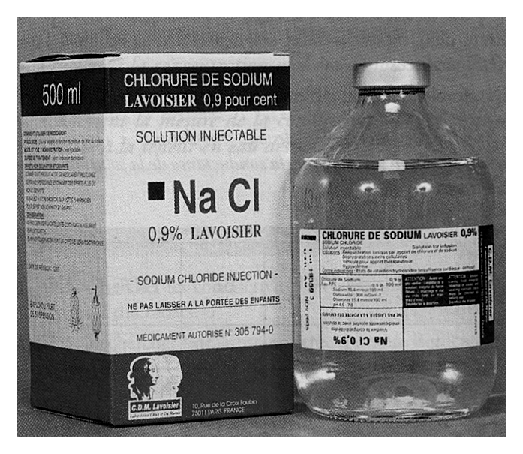
\includegraphics[width=7cm]{tp_prem_s_chimie/tp6_determination_par_conductimetrie_concentration/solution_nacl.png.eps}
\caption{Solution de chlorure de sodium}
\end{figure}
\end{center}


%\end{multicols}


\vressort{3}
\tp{D�termination par conductim�trie\\
de la concentration en solut�\\
d'une solution ionique}


\begin{multicols}{2}

\objectifs{
\item r�aliser une courbe d'�talonnage $G = f(C)$ et en d�duire une
  concentration inconnue.
\item Aborder une limite de la m�thode d'�talonnage.
}
\vspace*{2cm}


\materiel{
\item b�cher $600~mL$
\item fiole jaug�e $500~mL$
\item burette gradu�e $25~mL$
\item pipette jaug�e $5~mL$
\item agitateur magn�tique.
\item solution de chlorure de sodium $S_0$ de concentration $C_0 =
  0,10~mol.L^{-1}$
\item flacon de s�rum physiologique
\item eau d�min�ralis�e
\item g�n�rateur basse fr�quence.
\item 2 multim�tres
\item cellule de conductim�trie.
}


\end{multicols}




\section{R�alisation d'une �chelle de conductance}


\begin{multicols}{2}

\subsection{Protocole op�ratoire}
\begin{enumerate}
\item Rincer la burette, la remplir � l'aide de la solution $S_0$ ajuster le
z�ro.

\item Avec la fiole jaug�e, introduire $V = 500~mL$ d'eau d�min�ralis�e dans
le b�cher.

\item Placer la cellule conductim�trique dans le b�cher et r�aliser le
montage �lectrique correspondant au sch�ma ci-contre. Les 2
multim�tres sont en mode alternatif ($AC$ ou \acsymbol).

\item Sur le GBF, r�gler la fr�quence $500~Hz$ et fixer la tension �
$1,00~V$.

\item Au contenu du b�cher, ajouter les volumes $V_0$ suivants de solution
de chlorure de sodium mesur�s pr�cis�ment gr�ce � la burette. Apr�s
chaque addition, v�rifier que la tension est toujours de $1,00~V$ et
relever la valeur de l'intensit�.

\end{enumerate}




\begin{center}
\begin{figure}[H]
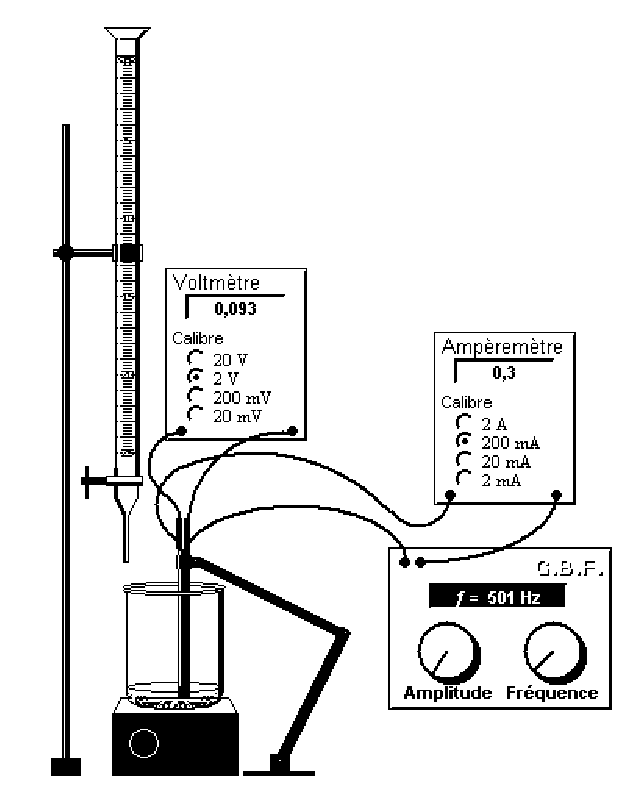
\includegraphics[width=6cm]{tp_prem_s_chimie/tp6_determination_par_conductimetrie_concentration/montage_conductimetrie.png.eps}
\caption{Dispositif exp�rimental}
\end{figure}
\end{center}


\end{multicols}



\subsection{R�sultats}
\begin{enumerate}
\item Calculer la conductance $G$ et compl�ter le tableau suivant.

\begin{arraydata}{6}
\hline
$V_0$ ($mL$)       &  0 &  5 & 10 & 15 & 20 & 25 \\ \hline
\rule[-0.4cm]{0cm}{1cm}
$C$ ($mol.L^{-1}$) &    &    &    &    &    &    \\ \hline
\rule[-0.4cm]{0cm}{1cm}
$G$ ($mS$)         &    &    &    &    &    &    \\ \hline
\end{arraydata}

\item Tracer la courbe d'�talonnage $G = f (C)$.
\end{enumerate}



\pagebreak
%\newpage


\section{D�termination de la concentration en $NaCl$ d'une solution de
  s�rum physiologique}

L'objectif est de d�terminer la concentration du chlorure de sodium dans le s�rum physiologique injectable.

\begin{enumerate}
\item Diluer au $1/100\ieme$ le s�rum physiologique. En pr�parer $500~mL$.

\item D�crire � l'aide de sch�mas le protocole utilis� pour r�aliser
  cette dilution au $1/100\ieme$ et obtenir la solution $S'$.

\item D�terminer la conductance $G'$ de cette solution $S'$.

\item En d�duire la concentration $C'$ du chlorure de sodium dans le
  s�rum physiologique dilu�.

\end{enumerate}


\vressort{3}

\section{Questions compl�mentaires}

%\begin{multicols}{2}

\begin{enumerate}
\item Expliquer comment calculer la concentration $C$ des diff�rentes
  solutions de chlorure de sodium. Donner l'expression de $C$ en
  fonction de $C_0$, $V_0$, $V$.


\item Comment calcule-t-on la conductance $G$ ?

\item Pour quelle raison pratique a-t-on int�r�t � prendre $U =
  1,00~V$ dans les diff�rentes manipulations ?

\item En extrapolant la courbe d'�talonnage, pr�voir la conductance
  d'une portion de solution concentr�e � $T = 58,4~g.L^{-1}$. Mesurer
  la conductance r�elle d'une portion d'une telle solution. Que
  peut-on conclure quant � la m�thode d'�talonnage utilis�e. On donne
  $M_{Na} = 23~g.mol^{-1}$ et $M_{Cl} = 35,5~g.mol^{-1}$.

\item Rappeler la valeur de la concentration $C'$ du chlorure de
  sodium dans le s�rum physiologique dilu�.

\item Comment peut-on alors d�terminer la concentration $C_0'$ du
  chlorure de sodium dans la solution commerciale de s�rum
  physiologique ? Calculer cette concentration $C_0'$ puis le titre
  massique (concentration massique) correspondant $T_0$. Le comparer avec
  les indications figurant sur l'�tiquette du flacon ($0,9~\%$ en masse).
\end{enumerate}


%\vressort{1}
\vressort{3}

\begin{center}
\begin{figure}[H]
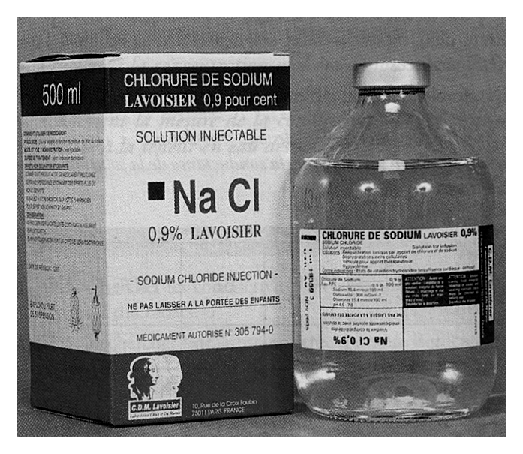
\includegraphics[width=7cm]{tp_prem_s_chimie/tp6_determination_par_conductimetrie_concentration/solution_nacl.png.eps}
\caption{Solution de chlorure de sodium}
\end{figure}
\end{center}


%\end{multicols}


\vressort{3}

\tp{D�termination par conductim�trie\\
de la concentration en solut�\\
d'une solution ionique}


\begin{multicols}{2}

\objectifs{
\item r�aliser une courbe d'�talonnage $G = f(C)$ et en d�duire une
  concentration inconnue.
\item Aborder une limite de la m�thode d'�talonnage.
}
\vspace*{2cm}


\materiel{
\item b�cher $600~mL$
\item fiole jaug�e $500~mL$
\item burette gradu�e $25~mL$
\item pipette jaug�e $5~mL$
\item agitateur magn�tique.
\item solution de chlorure de sodium $S_0$ de concentration $C_0 =
  0,10~mol.L^{-1}$
\item flacon de s�rum physiologique
\item eau d�min�ralis�e
\item g�n�rateur basse fr�quence.
\item 2 multim�tres
\item cellule de conductim�trie.
}


\end{multicols}




\section{R�alisation d'une �chelle de conductance}


\begin{multicols}{2}

\subsection{Protocole op�ratoire}
\begin{enumerate}
\item Rincer la burette, la remplir � l'aide de la solution $S_0$ ajuster le
z�ro.

\item Avec la fiole jaug�e, introduire $V = 500~mL$ d'eau d�min�ralis�e dans
le b�cher.

\item Placer la cellule conductim�trique dans le b�cher et r�aliser le
montage �lectrique correspondant au sch�ma ci-contre. Les 2
multim�tres sont en mode alternatif ($AC$ ou \acsymbol).

\item Sur le GBF, r�gler la fr�quence $500~Hz$ et fixer la tension �
$1,00~V$.

\item Au contenu du b�cher, ajouter les volumes $V_0$ suivants de solution
de chlorure de sodium mesur�s pr�cis�ment gr�ce � la burette. Apr�s
chaque addition, v�rifier que la tension est toujours de $1,00~V$ et
relever la valeur de l'intensit�.

\end{enumerate}




\begin{center}
\begin{figure}[H]
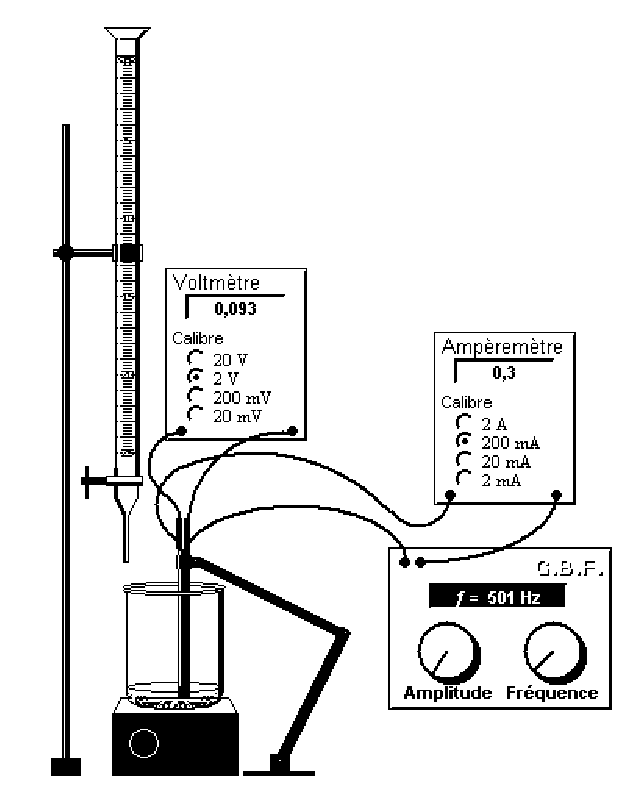
\includegraphics[width=6cm]{tp_prem_s_chimie/tp6_determination_par_conductimetrie_concentration/montage_conductimetrie.png.eps}
\caption{Dispositif exp�rimental}
\end{figure}
\end{center}


\end{multicols}



\subsection{R�sultats}
\begin{enumerate}
\item Calculer la conductance $G$ et compl�ter le tableau suivant.

\begin{arraydata}{6}
\hline
$V_0$ ($mL$)       &  0 &  5 & 10 & 15 & 20 & 25 \\ \hline
\rule[-0.4cm]{0cm}{1cm}
$C$ ($mol.L^{-1}$) &    &    &    &    &    &    \\ \hline
\rule[-0.4cm]{0cm}{1cm}
$G$ ($mS$)         &    &    &    &    &    &    \\ \hline
\end{arraydata}

\item Tracer la courbe d'�talonnage $G = f (C)$.
\end{enumerate}



\pagebreak
%\newpage


\section{D�termination de la concentration en $NaCl$ d'une solution de
  s�rum physiologique}

L'objectif est de d�terminer la concentration du chlorure de sodium dans le s�rum physiologique injectable.

\begin{enumerate}
\item Diluer au $1/100\ieme$ le s�rum physiologique. En pr�parer $500~mL$.

\item D�crire � l'aide de sch�mas le protocole utilis� pour r�aliser
  cette dilution au $1/100\ieme$ et obtenir la solution $S'$.

\item D�terminer la conductance $G'$ de cette solution $S'$.

\item En d�duire la concentration $C'$ du chlorure de sodium dans le
  s�rum physiologique dilu�.

\end{enumerate}


\vressort{3}

\section{Questions compl�mentaires}

%\begin{multicols}{2}

\begin{enumerate}
\item Expliquer comment calculer la concentration $C$ des diff�rentes
  solutions de chlorure de sodium. Donner l'expression de $C$ en
  fonction de $C_0$, $V_0$, $V$.


\item Comment calcule-t-on la conductance $G$ ?

\item Pour quelle raison pratique a-t-on int�r�t � prendre $U =
  1,00~V$ dans les diff�rentes manipulations ?

\item En extrapolant la courbe d'�talonnage, pr�voir la conductance
  d'une portion de solution concentr�e � $T = 58,4~g.L^{-1}$. Mesurer
  la conductance r�elle d'une portion d'une telle solution. Que
  peut-on conclure quant � la m�thode d'�talonnage utilis�e. On donne
  $M_{Na} = 23~g.mol^{-1}$ et $M_{Cl} = 35,5~g.mol^{-1}$.

\item Rappeler la valeur de la concentration $C'$ du chlorure de
  sodium dans le s�rum physiologique dilu�.

\item Comment peut-on alors d�terminer la concentration $C_0'$ du
  chlorure de sodium dans la solution commerciale de s�rum
  physiologique ? Calculer cette concentration $C_0'$ puis le titre
  massique (concentration massique) correspondant $T_0$. Le comparer avec
  les indications figurant sur l'�tiquette du flacon ($0,9~\%$ en masse).
\end{enumerate}


%\vressort{1}
\vressort{3}

\begin{center}
\begin{figure}[H]
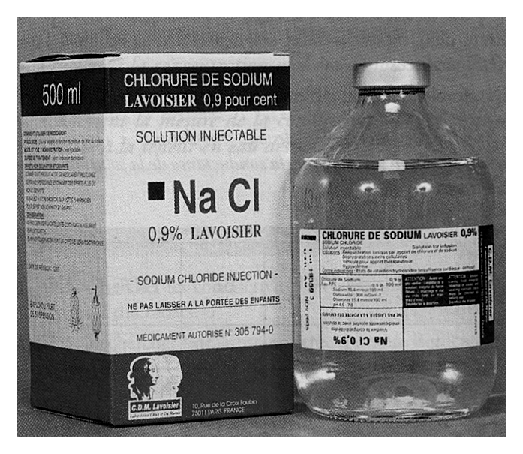
\includegraphics[width=7cm]{tp_prem_s_chimie/tp6_determination_par_conductimetrie_concentration/solution_nacl.png.eps}
\caption{Solution de chlorure de sodium}
\end{figure}
\end{center}


%\end{multicols}


\vressort{3}





%\chapitre{Thermique}
